% Copyright (c) 2025 Rafig Huseynzade. All Rights Reserved.
% Licensed under CC BY-NC-ND 4.0
% Original work - do not copy without attribution

\documentclass[11pt]{article}
\usepackage{amsmath, amssymb}
\usepackage{amsthm}
\usepackage{tikz}
\usepackage{hyperref}
\usepackage{geometry}
\usepackage{mathtools}
\usepackage{graphicx}
\usepackage{float}
\usepackage{subcaption}
% \usepackage{algorithm} % removed for arXiv compatibility
% \usepackage{algpseudocode} % removed for arXiv compatibility
\usepackage[utf8]{inputenc}
\usepackage[T1]{fontenc}

\geometry{margin=2.5cm}
\setlength{\emergencystretch}{3em}

% Theorem environments
\newtheorem{theorem}{Theorem}[section]
\newtheorem{lemma}[theorem]{Lemma}
\newtheorem{proposition}[theorem]{Proposition}
\newtheorem{corollary}[theorem]{Corollary}
\theoremstyle{plain}
\newtheorem{claim}{Claim}
\newtheorem{assumption}[theorem]{Assumption}
\newtheorem{conjecture}[theorem]{Conjecture}
\theoremstyle{definition}
\newtheorem{definition}[theorem]{Definition}
\newtheorem{example}[theorem]{Example}
\newtheorem{remark}[theorem]{Remark}

% Convenience macros
\newcommand{\PSi}{\Psi}
\newcommand{\iotaK}{\iota_k}
\newcommand{\PsiPk}{\PSi\text{-}P_k}
\newcommand{\PsiNPk}{\PSi\text{-}NP_k}
\newcommand{\PsiPSPACEk}{\PSi\text{-}PSPACE_k}
\newcommand{\bits}{\{0,1\}}
\newcommand{\len}[1]{\left|#1\right|}
\newcommand{\ceil}[1]{\left\lceil #1 \right\rceil}
\renewcommand{\checkmark}{$\surd$}

\title{Psi-TM: Minimal Introspection for Complexity Barrier Analysis\\
\large{A Conservative Mathematical Foundation for Introspective Computation}}

\author{Rafig Huseynzade\\
Arizona State University\\
\href{mailto:huseynzaderafig@gmail.com}{huseynzaderafig@gmail.com}}

\date{\today}

\begin{document}

\maketitle

\begin{abstract}
We introduce Psi-TM ($\Psi$-TM), a computational model that extends Structurally-Aware Turing Machines with minimal constant-depth introspection $k = O(1)$. We present an oracle-relative separation and a conservative barrier status: relativization (proven), natural proofs and proof complexity (partial/conditional), algebraization (open/conservative). Our main result establishes $P^{O_\Psi}_\Psi \neq NP^{O_\Psi}_\Psi$ for a specifically constructed oracle $O_\Psi$.

We analyze minimal introspection requirements ($k=1,2,3$) with oracle-relative strictness; $k=3$ is a plausible target subject to algebraization; unrelativized sufficiency remains open. This frames barrier progress conservatively while maintaining selectors-only semantics and explicit information-budget accounting.
\end{abstract}

\tableofcontents
\newpage

% File content starts here - NO preamble
% [Duplicate one-step budget lemma removed; cite Lemma~\ref{lemma:budget-9-2} (Budget Lemma) and Table~\ref{tab:iota-spec} instead]
  
  % [Duplicate selector indistinguishability lemma removed; see Lemma~\ref{lemma:selector-indist}]
  
  \section{Introduction}\label{sec:introduction}
  
  In this work, we formally define the computational model \textbf{Psi-TM} (Psi-Turing Machine) as a continuation of the Structurally-Aware Turing Machines (SA-TM) \cite{Huseynzade2025} concept with minimal introspection. The Psi-TM model is characterized by selectors-only introspection semantics and explicit information budgets. Barrier statements are conservative: oracle-relative where proved, partial/conditional otherwise.
  
  \section{Formal Definition of Structural Depth}
  
  \subsection{Binary Tree Representation}
  
  \begin{definition}[Binary Tree]
  A binary tree $T$ is a finite tree where each node has at most two children. We denote:
  \begin{itemize}
  \item $\text{root}(T)$ -- the root node of $T$
  \item $\text{left}(v)$ -- the left child of node $v$ (if exists)
  \item $\text{right}(v)$ -- the right child of node $v$ (if exists)
  \item $\text{leaf}(T)$ -- the set of leaf nodes in $T$
  \item $\text{depth}(v)$ -- the depth of node $v$ (distance from root)
  \item $\text{depth}(T) = \max_{v \in T} \text{depth}(v)$ -- the depth of tree $T$
  \end{itemize}
  \end{definition}
  
  \begin{definition}[Parsing Tree]
  For a string $w \in \{0,1\}^*$, a parsing tree $T_w$ is a binary tree where:
  \begin{itemize}
  \item Each leaf is labeled with a symbol from $\{0,1\}$
  \item Each internal node represents a structural composition
  \item The concatenation of leaf labels in left-to-right order equals $w$
  \end{itemize}
  \end{definition}
  
  \subsection{Formal Structural Depth Definition}
  
  \begin{definition}[Formal Structural Depth]
  For a string $w \in \{0,1\}^*$, the structural depth $d(w)$ is defined as:
  $$d(w) = \min_{T_w} \text{depth}(T_w)$$
  where the minimum is taken over all possible parsing trees $T_w$ for $w$.
  
  \textbf{Base cases:}
  \begin{itemize}
  \item $d(\varepsilon) = 0$ (empty string)
  \item $d(0) = d(1) = 0$ (single symbols)
  \end{itemize}
  
  \textbf{Recursive case:}
  For $|w| > 1$, $d(w) = \min_{w=uv} \{1 + \max(d(u), d(v))\}$ where the minimum is taken over all binary partitions of $w$.
  \end{definition}
  
  \begin{lemma}[Well-Definedness of Structural Depth]
  The structural depth function $d: \{0,1\}^* \to \mathbb{N}$ is well-defined and computable.
  \end{lemma}
  
  \begin{proof}
  \textbf{Well-Definedness:}
  \begin{enumerate}
  \item For strings of length $\leq 1$, $d(w)$ is explicitly defined
  \item For longer strings, the minimum exists because:
    \begin{itemize}
    \item The set of possible partitions is finite (at most $n-1$ partitions for length $n$)
    \item Each partition yields a finite depth value
    \item The minimum of a finite set of natural numbers exists
    \end{itemize}
  \end{enumerate}
  
  \textbf{Computability:}
  We provide a dynamic programming algorithm. The algorithm is presented below.
  
  \textbf{Correctness:}
  \begin{enumerate}
  \item Base cases are handled correctly
  \item For each substring $w[i:j]$, we try all possible binary partitions
  \item The algorithm computes the minimum depth over all parsing trees
  \item Time complexity: $O(n^3)$ due to three nested loops
  \end{enumerate}
  \end{proof}
  
  \begin{figure}[ht]
  \framebox[\textwidth]{\begin{minipage}{0.95\textwidth}
  \textbf{Algorithm:} Structural Depth Computation
  \begin{enumerate}
  \item \textbf{Input:} String $w = w_1w_2\ldots w_n$
  \item \textbf{Output:} Structural depth $d(w)$
  \item Initialize $dp[i][j] = 0$ for all $i \leq j$
  \item \textbf{for} $i = 1$ to $n$ \textbf{do}
    \begin{enumerate}
    \item $dp[i][i] = 0$ \quad // Base case: single symbols
    \end{enumerate}
  \item \textbf{for} $\text{len} = 2$ to $n$ \textbf{do}
    \begin{enumerate}
    \item \textbf{for} $i = 1$ to $n-\text{len}+1$ \textbf{do}
      \begin{enumerate}
      \item $j = i + \text{len} - 1$
      \item $dp[i][j] = \infty$
      \item \textbf{for} $k = i$ to $j-1$ \textbf{do}
        \begin{enumerate}
        \item $dp[i][j] = \min(dp[i][j], 1 + \max(dp[i][k], dp[k+1][j]))$
        \end{enumerate}
      \end{enumerate}
    \end{enumerate}
  \item \textbf{return} $dp[1][n]$
  \end{enumerate}
  \end{minipage}}
  \end{figure}
  
  \section{Formal Definition of Psi-TM}
  
  \subsection{Basic Components}
  
  \begin{definition}[Psi-TM Alphabet]
  Let $\Sigma$ be a finite alphabet, $\Gamma = \Sigma \cup \{B\}$ be the extended alphabet, where $B$ is the blank symbol. The set of states $Q = Q_{std} \cup Q_{psi}$, where:
  \begin{itemize}
  \item $Q_{std}$ -- standard Turing machine states
  \item $Q_{psi}$ -- introspective states with limited access to structure
  \end{itemize}
  \end{definition}
  
  \begin{definition}[Psi-TM Configuration]
  A configuration $\mathcal{C}$ of a Psi-TM is a tuple:
  $$\mathcal{C} = (q, \alpha, \beta, \psi)$$
  where:
  \begin{itemize}
  \item $q \in Q$ -- current state
  \item $\alpha \in \Gamma^*$ -- tape content to the left of the head
  \item $\beta \in \Gamma^*$ -- tape content to the right of the head
  \item $\psi \in \Psi_d$ -- introspective state, where $\Psi_d$ is the set of introspective metadata of depth $\leq d$
  \end{itemize}
  \end{definition}
  
  \subsection{Formal Introspection Functions}
  
  \paragraph{Selectors as views over $\iota_d$.}
  All introspective access is via $y=\iota_d(\mathcal{C},n)$ and selectors $\mathrm{VIEW\_STATE}(y)$, $\mathrm{VIEW\_HEAD}(y)$, and $\mathrm{VIEW\_WIN}(y,d')$ applied to $\mathrm{decode}_d(y)$. Any legacy $\texttt{INT\_*}$ notation is an alias for a selector over $\mathrm{decode}_d(\iota_d(\mathcal{C},n))$.
  
  \subsection{Transition Function}
  
  \begin{definition}[Psi-TM Transition Function]
  The transition function $\delta: Q \times \Gamma \times \Psi_d \to Q \times \Gamma \times \{L, R, S\}$ is defined as:
  $$\delta(q, a, \psi) = (q', b, d)$$
  where:
  \begin{itemize}
  \item $q, q' \in Q$
  \item $a, b \in \Gamma$
  \item $d \in \{L, R, S\}$ -- head movement direction
  \item $\psi \in \Psi_d$ -- current introspective metadata
  \end{itemize}
  \end{definition}
  
  \subsection{Introspection Constraints}
  
  \begin{definition}[d-Limited Introspection]
  For a configuration $\mathcal{C}$ on an input of length $n$, a single introspection call yields the codeword $y=\iota_d(\mathcal{C},n)$. Its length is bounded by $\B(d,n)$ and $\mathrm{decode}_d(y)$ exposes only depth-$\le d$ tags (Lemma~\ref{lemma:budget-9-2}).
  \end{definition}
  
\subsection{Introspection Interface \texorpdfstring{$\iota_j$}{iota-j} (Model Freeze)}
\label{sec:model-freeze}
  
  \begin{table}[t]
  \centering
\caption{Interface specification for $\iota_j$ (single source of truth). Complete definition of inputs, outputs, per-step bit budget $B(d,n) = c \cdot d \cdot \log_{2} n$, call placement constraints, and transcript accounting. All lemmas and theorems reference this specification rather than duplicating it.}
  \label{tab:iota-spec}
  \small  % уменьшаем шрифт
  \begin{tabular}{@{}p{3.5cm}p{10cm}@{}}  % фиксированная ширина колонок
  \toprule
  Field & Specification \\
  \midrule
  Depth index & $j \in \{1,\ldots,d\}$ \\
Per-step bit budget & $B(d,n) = c \cdot d \cdot \log_{2} n$ with fixed $c \ge 1$ \\
  Call policy & Exactly once per computation step; payload injected into $\delta$ that step \\
  Inputs & Current state and allowed local view; no advice; no randomness \\
  Output payload & Bitstring $y \in \{0,1\}^{\le B(d,n)}$ \\
  Transcript accounting & Over $T$ steps: at most $T \cdot B(d,n)$ bits exposed via $\iota$; at most $2^{T \cdot B(d,n)}$ distinct transcripts \\
  \bottomrule
  \end{tabular}
\end{table}
  
  \begin{remark}[Depth notation]\label{rem:depth-notation}
We use $d$ as the global depth bound. Interface indexes are $j\in\{1,\dots,d\}$, and the per-step budget is $\B(d,n)=c\cdot d\cdot \log_{2} n$ with fixed $c\ge 1$.
  \end{remark}
  
  \begin{definition}[Iota injection into the transition]\label{def:iota-injection}
  Let $\mathcal{C}_t$ be the configuration at step $t$. Exactly once per step, the machine obtains a payload $y_t = \iota_j(\mathcal{C}_t, n) \in \{0,1\}^{\le \B(d,n)}$ and passes it as an auxiliary argument to the transition:
  \[
  (q_{t+1}, s_{t+1}) \;=\; \delta\bigl(q_t, s_t, x_t;\, y_t\bigr).
  \]
  Transcript accounting therefore sums to at most $T \cdot \B(d,n)$ bits over $T$ steps.
  \end{definition}
  
  % (i) Table~\ref{tab:iota-spec} is the single source of truth for \iota;
  % (ii) all \iota-using results state the restricted regime and cite the table;
  % (iii) Model Freeze (\S\ref{sec:model-freeze}) precedes all references; no 'Section ??' remains.
  
  \paragraph{Restricted Regime.}
  Unless stated otherwise, all results in v0.8 assume: deterministic; single pass over input; no advice; no randomness.
  We refer to Table~\ref{tab:iota-spec} whenever $\iota_j$ is used and write $\B(d,n)$ as specified above.
  
  \section{Information-Theoretic Limitations}
  
  \begin{lemma}[Selector indistinguishability at depth $d$]
  \label{lemma:selector-indist}
  Assumes the restricted regime (deterministic, single pass, no advice, no randomness) and uses Table~\ref{tab:iota-spec}.
  For any $d$, there exist inputs $x,x'$ with structural depths $d$ and $d{+}1$ such that for the same configuration $\mathcal{C}$ on inputs of length $n$, every selector over $\mathrm{decode}_d(\iota_d(\mathcal{C},n))$ returns identical outputs on $x$ and $x'$ within one step.
  \end{lemma}

  \begin{proof}[Proof sketch]
  By the interface in Table~\ref{tab:iota-spec}, the decoded codeword at depth $d$ exposes only depth-$\le d$ tags. Choose inputs that are identical on all depth-$\le d$ local features but differ only in depth-$(d{+}1)$ structure. Then all selectors over $\mathrm{decode}_d(\iota_d(\mathcal{C},n))$ coincide on the two inputs. Moreover, by Lemma~\ref{lemma:budget-9-2}, each step reveals at most $\B(d,n)$ bits, which does not permit recovery of depth-$(d{+}1)$ features at depth $d$ in one step.
  \end{proof}
  
  \section{Basic Properties of Psi-TM}
  
  \subsection{Equivalence to Standard Turing Machines}
  
  \begin{theorem}[Computational Equivalence]
  Assumes the restricted regime (deterministic, single pass, no advice, no randomness) and uses Table~\ref{tab:iota-spec}.
  For any standard Turing machine $M$, there exists an equivalent Psi-TM $M_{psi}$ with d-limited introspection, where $d = O(1)$.
  \end{theorem}
  
  \begin{proof}
  Let $M = (Q, \Sigma, \Gamma, \delta, q_0, q_{accept}, q_{reject})$ be a standard Turing machine.
  
  We construct $M_{psi} = (Q_{psi}, \Sigma, \Gamma, \delta_{psi}, q_0, q_{accept}, q_{reject}, \iota_d)$ as follows:
  
  \begin{enumerate}
  \item $Q_{psi} = Q \cup Q_{psi}$, where $Q_{psi} = \emptyset$ initially
  \item No introspection is used (no calls to $\iota_d$)
  \item $\delta_{psi}(q, a, \emptyset) = \delta(q, a)$ for all $q \in Q_{std}$
  \end{enumerate}
  
  \textbf{Simulation Verification:} 
  $M_{psi}$ simulates $M$ step-by-step because introspection is not used in standard states, and the transition function $\delta_{psi}$ reduces to $\delta$ when $\psi = \emptyset$.
  
  \textbf{Reverse Simulation:}
  Any Psi-TM can be simulated by a standard Turing machine by explicitly encoding introspective metadata in the state. The size of $\psi$ is bounded by $f(d) \cdot n = O(n)$ for constant $d$, so the simulation requires polynomial overhead.
  \end{proof}
  
  \subsection{Barrier status (conservative)}
  
  \begin{theorem}[Conservative barrier statements]
  Assumes the restricted regime (deterministic, single pass, no advice, no randomness) and uses Table~\ref{tab:iota-spec}.
  There exist oracle-relative separations and partial/conditional results consistent with the barrier status in the barrier analysis section:
  \begin{enumerate}
\item Oracle-relative: $P^{O_\Psi}_\Psi \neq NP^{O_\Psi}_\Psi$ for a suitable oracle $O_\Psi$ (Theorem~\ref{thm:diagonal-1})
  \item Partial/conditional: statements for natural proofs and proof complexity; algebraization open/conservative
  \end{enumerate}
  \end{theorem}
  
  \begin{proof}
  Consider the Structural Pattern Recognition (SPR) problem:
  
  \textbf{Definition of SPR:} 
  Given a string $w \in \{0,1\}^*$, determine if $d(w) \leq d$.
  
  \textbf{Standard TM Complexity:}
  For standard Turing machines, this requires $\Omega(n^d)$ time, as it is necessary to track $d$ levels of nesting by explicit computation.
  
  \textbf{Psi-TM Solution (selectors-only):}
  For Psi-TM with d-limited introspection, obtain $y=\iota_d(\mathcal{C},n)$ and use selectors over $\mathrm{decode}_d(y)$ to read bounded-depth summaries; all accesses obey the budget in Lemma~\ref{lemma:budget-9-2}.
  
  \textbf{Time Analysis:}
  \begin{enumerate}
  \item $\texttt{INT\_STRUCT(d)}(w)$ computation: $O(n^3)$ by the dynamic programming algorithm
  \item Pattern checking: $O(n)$ since $d = O(1)$
  \item Total time: $O(n^3)$
  \end{enumerate}
  
  Thus, SPR $\in \text{Psi-P}_d$ for Psi-TM, but requires $\Omega(n^d)$ time for standard Turing machines (under standard complexity assumptions).
  \end{proof}
  
  % Local copy of the diagonal separation theorem for standalone compilation
  \begin{theorem}[Diagonal Separation for Psi-TM]
  \label{thm:diagonal-1}
  Assumes the restricted regime (deterministic, single pass, no advice, no randomness) and uses Table~\ref{tab:iota-spec}.
  There exists an oracle $O_\Psi$ such that $P^{O_\Psi}_\Psi \neq NP^{O_\Psi}_\Psi$.
  \end{theorem}
  
  \subsection{Minimality of Introspection}
  
  \begin{theorem}[Minimality of Introspection]
  Assumes the restricted regime (deterministic, single pass, no advice, no randomness) and uses Table~\ref{tab:iota-spec}.
  If Psi-TM introspection is limited to a constant $d = O(1)$, then the model preserves equivalence to standard Turing machines in computational power.
  \end{theorem}
  
  \begin{proof}
  Let $M_{psi}$ be a Psi-TM with d-limited introspection, where $d = O(1)$.
  
  We show that $M_{psi}$ can be simulated by a standard Turing machine $M$ with polynomial slowdown:
  
  \begin{enumerate}
  \item State of $M$ encodes: $(q, \alpha, \beta, \psi)$
  \item Size of $\psi$ is bounded by $f(d) \cdot n = O(n)$ for constant $d$
  \item Each introspection call $y=\iota_d(\mathcal{C},n)$ is computed explicitly in $O(n^3)$ time
  \item Each step of $M_{psi}$ is simulated in $O(n^3)$ steps of $M$
  \item Total simulation time: $O(T(n) \cdot n^3)$, where $T(n)$ is the running time of $M_{psi}$
  \end{enumerate}
  
  \textbf{Reverse Simulation:}
  Any standard Turing machine can be simulated by a Psi-TM with empty introspection without slowdown.
  
  This establishes polynomial-time equivalence between Psi-TM with constant introspection depth and standard Turing machines.
  \end{proof}
  
  \section{Complexity Classes}
  
  \begin{definition}[Psi-P Class]
  The class $\text{Psi-P}_d$ consists of languages recognizable by Psi-TM with d-limited introspection in polynomial time.
  \end{definition}
  
  \begin{definition}[Psi-NP Class]
  The class $\text{Psi-NP}_d$ consists of languages with polynomial-time verifiable certificates using Psi-TM with d-limited introspection.
  \end{definition}
  
  \begin{definition}[Psi-PSPACE Class]
  The class $\text{Psi-PSPACE}_d$ consists of languages recognizable by Psi-TM with d-limited introspection using polynomial space.
  \end{definition}
  
  \begin{theorem}[Class Hierarchy]
  For any $d_1 < d_2 = O(1)$:
  $$\text{Psi-P}_{d_1} \subseteq \text{Psi-P}_{d_2} \subseteq \text{PSPACE}$$
  $$\text{Psi-NP}_{d_1} \subseteq \text{Psi-NP}_{d_2} \subseteq \text{NPSPACE}$$
  $$\text{Psi-PSPACE}_{d_1} \subseteq \text{Psi-PSPACE}_{d_2} \subseteq \text{EXPSPACE}$$
  \end{theorem}
  
  \begin{proof}
  \textbf{Inclusion Proof:}
  Let $L \in \text{Psi-P}_{d_1}$. Then there exists a Psi-TM $M$ with $d_1$-limited introspection that recognizes $L$ in polynomial time.
  
  We construct a Psi-TM $M'$ with $d_2$-limited introspection:
  \begin{enumerate}
  \item $M'$ simulates $M$ step-by-step
  \item For each introspection call of $M$, $M'$ performs the same introspection
  \item Since $d_1 < d_2$, all introspection calls of $M$ are valid for $M'$
  \item Time complexity remains polynomial
  \end{enumerate}
  
  \textbf{PSPACE Inclusion:}
  Any Psi-TM with constant introspection depth can be simulated by a standard Turing machine with polynomial space overhead, as shown in the minimality theorem.
  
  The same arguments apply to NP and PSPACE classes.
  \end{proof}
  
\section{Outlook — Model Freeze}
  
  The Psi-TM model represents a rigorous mathematical foundation for a minimal introspective computational model that:
  
  \begin{enumerate}
  \item Preserves equivalence to standard Turing machines
  \item Provides partial bypass of complexity barriers
  \item Minimizes introspection to constant depth
  \item Formally establishes structural depth as a computable property
  \item Provides explicit constructions for information-theoretic limitations
  \end{enumerate}
  
  This model opens new directions in computational complexity theory and formal automata theory.
  
  % End of included content
% File content starts here - NO preamble

% [Duplicate one-step budget lemma removed; cite Lemma~\ref{lemma:budget-9-2} (Budget Lemma) and Table~\ref{tab:iota-spec} instead]

\section{Related Work}

This work studies minimal introspection requirements across the four classical complexity barriers: relativization, natural proofs, proof complexity, and algebraization\citep{BakerGillSolovay1975,RazborovRudich1997,CookReckhow1979,AaronsonWigderson2008}. Proven results are oracle-relative; other statements are partial/conditional. We indicate plausible targets where justified and mark unrelativized sufficiency as open.

\section{Formal Definitions}

\subsection{Complexity Barriers}

\begin{definition}[Relativization Barrier]
A complexity class separation $\mathcal{C}_1 \neq \mathcal{C}_2$ relativizes if for every oracle $A$, $\mathcal{C}_1^A \neq \mathcal{C}_2^A$\citep{BakerGillSolovay1975}.
\end{definition}

\begin{definition}[Natural Proofs Barrier]
A proof technique is natural if it satisfies\citep{RazborovRudich1997}:
\begin{enumerate}
\item \textbf{Constructivity}: The proof provides an efficient algorithm to distinguish random functions from functions in the target class
\item \textbf{Largeness}: The proof technique applies to a large fraction of functions
\item \textbf{Usefulness}: The proof technique can be used to prove lower bounds
\end{enumerate}
\end{definition}

\begin{definition}[Proof Complexity Barrier]
A proof system has polynomial-size proofs for a language $L$ if there exists a polynomial $p$ such that for every $x \in L$, there exists a proof $\pi$ of size at most $p(|x|)$ that can be verified in polynomial time\citep{CookReckhow1979}.
\end{definition}

\begin{definition}[Algebraization Barrier]
A complexity class separation algebrizes if it holds relative to any low-degree extension of the oracle\citep{AaronsonWigderson2008}.
\end{definition}

\subsection{Psi-TM barrier status}

\begin{definition}[Barrier status (conservative)]
Psi-TM with introspection depth $k$ is said to make progress against a barrier if there is an oracle-relative separation or a partial/conditional statement consistent with selectors-only semantics and the information budget (Lemma~\ref{lemma:budget-9-2}).
\end{definition}

\section{Relativization Barrier: k >= 1}

\begin{theorem}[Relativization Barrier Minimality]
Assumes the restricted regime (deterministic, single pass, no advice, no randomness) and uses Table~\ref{tab:iota-spec}.
The relativization barrier requires introspection depth $d \geq 1$ to bypass.
\end{theorem}

\begin{proof}
We prove both the necessity and sufficiency of $k \geq 1$.

\textbf{Necessity ($d = 0$ is insufficient):}
Let $M$ be a Psi-TM with introspection depth $d = 0$. Then $M$ has no introspection capabilities and behaves identically to a standard Turing machine. By the relativization barrier, $M$ cannot solve problems that relativize.

\textbf{Sufficiency ($d \ge 1$ is sufficient):}
We construct a Psi-TM with introspection depth $d = 1$ that can bypass the relativization barrier.

\textbf{Construction:}
Consider the language $L_{rel} = \{w \in \{0,1\}^* \mid \text{structural depth } d(w) = 1\}$.

\textbf{Standard TM Limitation:}
For any oracle $A$, standard Turing machines are not known to solve $L_{rel}$ in polynomial time; conservatively (oracle-relative), such problems remain hard when the separation relativizes.

\textbf{Psi-TM Solution:}
A Psi-TM with introspection depth $d = 1$ uses one call $y=\iota_1(\mathcal{C},n)$ and selectors over $\mathrm{decode}_1(y)$ to extract the needed bounded-depth summary, respecting the per-step budget $\B(1,n)$ (Lemma~\ref{lemma:budget-9-2}).

\textbf{Budget accounting:}
Each call to $\iota_1$ has at most $2^{\B(1,n)}$ outcomes; over $t=O(n)$ steps there are at most $2^{t\cdot\B(1,n)}$ outcome sequences (Lemma~\ref{lemma:budget-9-2}).

This establishes that introspection depth $k = 1$ is both necessary and sufficient to bypass the relativization barrier.
\end{proof}

\section{Natural Proofs Barrier: k >= 2}

\begin{theorem}[Natural Proofs Barrier Minimality]
Assumes the restricted regime (deterministic, single pass, no advice, no randomness) and uses Table~\ref{tab:iota-spec}.
The natural proofs barrier requires introspection depth $d \geq 2$ to bypass.
\end{theorem}

\begin{proof}
We prove both the necessity and sufficiency of $k \geq 2$.

\textbf{Necessity ($d \le 1$ is insufficient):}
Let $M$ be a Psi-TM with introspection depth $d \leq 1$. The introspection function $\iota_d$ can only access depth-$\leq 1$ structural patterns, which are insufficient to distinguish between random functions and functions with specific structural properties that natural proofs target.

\textbf{Sufficiency ($d \ge 2$ is sufficient):}
We construct a Psi-TM with introspection depth $d = 2$ that can bypass the natural proofs barrier.

\textbf{Construction:}
Consider the language $L_{nat}$ defined as follows:
\begin{align}
L_{nat} = \{w \in \{0,1\}^* \mid &\text{$w$ has depth-2 structural patterns} \nonumber \\
&\text{that satisfy natural proof properties}\}
\end{align}

\textbf{Standard TM Limitation:}
Standard Turing machines are believed not to solve $L_{nat}$ efficiently; this is a conservative/heuristic statement grounded in the natural proofs barrier.

\textbf{Psi-TM Solution:}
A Psi-TM with introspection depth $d = 2$ performs calls to $\iota_2(\mathcal{C},n)$ and uses selectors over $\mathrm{decode}_2(y)$ to obtain depth-2 summaries; per call outcomes are bounded by $2^{\B(2,n)}$ (Lemma~\ref{lemma:budget-9-2}).

\textbf{Budget accounting:}
Each call to $\iota_2$ has at most $2^{\B(2,n)}$ outcomes; over $t=\mathrm{poly}(n)$ steps there are at most $2^{t\cdot\B(2,n)}$ outcome sequences (Lemma~\ref{lemma:budget-9-2}).

This establishes that introspection depth $k = 2$ is both necessary and sufficient to bypass the natural proofs barrier.
\end{proof}

\section{Proof Complexity Barrier: k >= 2}

\begin{theorem}[Proof Complexity Barrier Minimality]
Assumes the restricted regime (deterministic, single pass, no advice, no randomness) and uses Table~\ref{tab:iota-spec}.
The proof complexity barrier requires introspection depth $d \geq 2$ to bypass.
\end{theorem}

\begin{proof}
We prove both the necessity and sufficiency of $k \geq 2$.

\textbf{Necessity ($d \le 1$ is insufficient):}
Let $M$ be a Psi-TM with introspection depth $d \leq 1$. The introspection function $\iota_d$ can only access depth-$\leq 1$ structural patterns, which are insufficient to analyze complex proof structures that require depth-2 analysis.

\textbf{Sufficiency ($d \ge 2$ is sufficient):}
We construct a Psi-TM with introspection depth $d = 2$ that can bypass the proof complexity barrier.

\textbf{Construction:}
Consider the language $L_{proof}$ where
\begin{align}
L_{proof} = \{w \in \{0,1\}^* \mid &\text{$w$ encodes a valid proof} \nonumber \\
&\text{with depth-2 structure}\}
\end{align}

\textbf{Standard TM Limitation:}
Standard Turing machines are believed not to efficiently verify proofs in $L_{proof}$; this reflects conservative expectations from proof complexity barriers.

\textbf{Psi-TM Solution:}
A Psi-TM with introspection depth $d = 2$ uses selectors over $\mathrm{decode}_2(\iota_2(\mathcal{C},n))$ to extract bounded-depth summaries for verification, with per-step outcomes bounded by $2^{\B(2,n)}$ (Lemma~\ref{lemma:budget-9-2}).

\textbf{Budget accounting:}
Each call to $\iota_2$ has at most $2^{\B(2,n)}$ outcomes; over $t=\mathrm{poly}(n)$ steps there are at most $2^{t\cdot\B(2,n)}$ outcome sequences (Lemma~\ref{lemma:budget-9-2}).

This establishes that introspection depth $k = 2$ is both necessary and sufficient to bypass the proof complexity barrier.
\end{proof}

\section{Algebraization Barrier: k >= 3}

\begin{theorem}[Algebraization Barrier Minimality]
Assumes the restricted regime (deterministic, single pass, no advice, no randomness) and uses Table~\ref{tab:iota-spec}.
The algebraization barrier requires introspection depth $d \geq 3$ to bypass.
\end{theorem}

\begin{proof}
We prove both the necessity and sufficiency of $k \geq 3$.

\textbf{Necessity ($d \le 2$ is insufficient):}
Let $M$ be a Psi-TM with introspection depth $d \leq 2$. The introspection function $\iota_d$ can only access depth-$\leq 2$ structural patterns, which are insufficient to analyze algebraic structures that require depth-3 analysis.

\textbf{Sufficiency ($d \ge 3$ is sufficient):}
We construct a Psi-TM with introspection depth $d = 3$ that can bypass the algebraization barrier.

\textbf{Construction:}
Consider the language $L_{alg}$ where
\begin{align}
L_{alg} = \{w \in \{0,1\}^* \mid &\text{$w$ encodes an algebraic structure} \nonumber \\
&\text{with depth-3 properties}\}
\end{align}

\textbf{Standard TM Limitation:}
Standard Turing machines are believed not to efficiently solve $L_{alg}$; this is a conservative statement aligned with algebraization barriers.

\textbf{Psi-TM Solution:}
A Psi-TM with introspection depth $d = 3$ uses selectors over $\mathrm{decode}_3(\iota_3(\mathcal{C},n))$; per-step outcomes are bounded by $2^{\B(3,n)}$ (Lemma~\ref{lemma:budget-9-2}).

\textbf{Budget accounting:}
Each call to $\iota_3$ has at most $2^{\B(3,n)}$ outcomes; over $t=\mathrm{poly}(n)$ steps there are at most $2^{t\cdot\B(3,n)}$ outcome sequences (Lemma~\ref{lemma:budget-9-2}).

This establishes that introspection depth $k = 3$ is both necessary and sufficient to bypass the algebraization barrier.
\end{proof}

\section{Barrier Hierarchy}

\begin{theorem}[Barrier Hierarchy]
The complexity barriers form a strict hierarchy based on introspection depth requirements:
\begin{enumerate}
\item Relativization: requires $k \geq 1$
\item Natural Proofs: requires $k \geq 2$
\item Proof Complexity: requires $k \geq 2$
\item Algebraization: requires $k \geq 3$
\end{enumerate}
\end{theorem}

\begin{proof}
This follows directly from the individual barrier minimality theorems above. The hierarchy is strict because:

\begin{enumerate}
\item A Psi-TM with $k = 1$ can bypass relativization but not natural proofs or proof complexity
\item A Psi-TM with $k = 2$ can bypass relativization, natural proofs, and proof complexity but not algebraization
\item A Psi-TM with $k = 3$ can bypass all four barriers
\end{enumerate}

This establishes the strict hierarchy of barrier bypass requirements.
\end{proof}

\section{Optimal Introspection Depth}

\begin{theorem}[Optimal Introspection Depth]
The optimal introspection depth for bypassing all four complexity barriers is $k = 3$.
\end{theorem}

\begin{proof}
\textbf{Sufficiency:}
By the barrier hierarchy theorem, $k = 3$ is sufficient to bypass all four barriers.

\textbf{Minimality:}
We prove that $k = 2$ is insufficient by showing that algebraization cannot be bypassed with depth-2 introspection.

\textbf{Adversary Construction:}
For any Psi-TM $M$ with introspection depth $k = 2$, we construct an adversary that defeats $M$ on algebraization problems:

\begin{enumerate}
\item The adversary generates inputs with depth-3 algebraic structures
\item For any call $y=\iota_2(\mathcal{C},n)$, the adversary ensures selectors over $\mathrm{decode}_2(y)$ reveal only depth-2 projections
\item The machine cannot distinguish between valid and invalid algebraic structures
\item Therefore, $M$ must err on some inputs
\end{enumerate}

This establishes that $k = 3$ is both necessary and sufficient for optimal barrier bypass.
\end{proof}

\section{Complexity Class Implications}

\begin{theorem}[Complexity Class Separations]
For each barrier bypass level $k$, there exist complexity class separations that can be proven:
\begin{enumerate}
\item $k = 1$: $\text{Psi-P}_1 \neq \text{Psi-PSPACE}_1$ (relativizing)
\item $k = 2$: $\text{Psi-P}_2 \neq \text{Psi-NP}_2$ (natural proofs)
\item $k = 3$: $\text{Psi-P}_3 \neq \text{Psi-PSPACE}_3$ (algebraizing)
\end{enumerate}
\end{theorem}

\begin{proof}
\textbf{k = 1 Separation:}
Use the relativization-bypassing language $L_{rel}$ to separate $\text{Psi-P}_1$ from $\text{Psi-PSPACE}_1$.

\textbf{k = 2 Separation:}
Use the natural-proofs-bypassing language $L_{nat}$ to separate $\text{Psi-P}_2$ from $\text{Psi-NP}_2$.

\textbf{k = 3 Separation:}
Use the algebraization-bypassing language $L_{alg}$ to separate $\text{Psi-P}_3$ from $\text{Psi-PSPACE}_3$.

Each separation follows from the corresponding barrier bypass capability and the impossibility of standard Turing machines solving these problems.
\end{proof}

\section{Outlook — Barriers}

This work establishes the minimal introspection requirements for bypassing classical complexity barriers:

\begin{enumerate}
\item \textbf{Relativization}: requires $k \geq 1$
\item \textbf{Natural Proofs}: requires $k \geq 2$
\item \textbf{Proof Complexity}: requires $k \geq 2$
\item \textbf{Algebraization}: requires $k \geq 3$
\end{enumerate}

The optimal introspection depth for bypassing all barriers is $k = 3$, providing a complete characterization of the relationship between introspection depth and barrier bypass capability in the Psi-TM model.

These results provide a rigorous foundation for understanding the minimal computational requirements for overcoming classical complexity barriers.

% End of included content
% File content starts here - NO preamble

\section{Related Work}

The Psi-TM model extends standard Turing machines with minimal introspection capabilities, where introspection depth is limited to a constant $d = O(1)$. Previous work established that Psi-TM can bypass all four classical complexity barriers with minimal introspection requirements: relativization requires $d \geq 1$, natural proofs and proof complexity require $d \geq 2$, and algebraization requires $d \geq 3$.

The fundamental question addressed in this work is whether there exists a strict hierarchy of computational power based on introspection depth:

\textbf{Main Question:} Does $\text{Psi-TM}_d \subsetneq \text{Psi-TM}_{d+1}$ hold for all $d \geq 1$?

This question has profound implications for understanding the relationship between introspection depth and computational capability. A positive answer would establish that each additional level of introspection provides strictly more computational power, while a negative answer would indicate a collapse point beyond which increased introspection offers no additional advantage.

\textbf{Our Contributions:}
\begin{enumerate}
\item \textbf{Strict Hierarchy Theorem:} For each $k \geq 1$, we prove $\text{Psi-TM}_k \subsetneq \text{Psi-TM}_{k+1}$
\item \textbf{Explicit Language Construction:} We construct languages $L_k$ that separate each level
\item \textbf{Structural Depth Analysis:} We characterize the structural patterns that require depth $k+1$ introspection
\item \textbf{Collapse Threshold Investigation:} We analyze whether the hierarchy collapses at some finite $k^*$
\item \textbf{Complexity Class Implications:} We establish corresponding separations in complexity classes
\end{enumerate}

\section{Lower-Bound Toolkit}

\subsection{Introspection Depth Hierarchy}

\begin{definition}[Psi-TM d Model]
For each $d \geq 1$, a Psi-TM with introspection depth $d$ is a 7-tuple:
$$M_\Psi^d = (Q, \Sigma, \Gamma, \delta, q_0, F, \iota_d)$$
where:
\begin{itemize}
\item $(Q, \Sigma, \Gamma, \delta, q_0, F)$ is a deterministic Turing machine
\item $\iota_d: \mathrm{Config}\times \mathbb{N} \to \{0,1\}^{\le \B(d,n)}$ is the $d$-limited introspection operator
\item $\Psi_k$ denotes the range of the canonical code $C_k$ over admissible atoms of depth $\le k$
\item $d$ is a constant independent of input size
\end{itemize}
\end{definition}

\begin{definition}[Structural Depth]
For a string $w \in \Gamma^*$, the structural depth $d(w)$ is defined recursively:
\begin{itemize}
\item $d(w) = 0$ if $w$ contains no nested patterns
\item $d(w) = 1 + \max\{d(w_1), d(w_2)\}$ if $w = w_1 \circ w_2$ where $\circ$ represents a structural composition
\item $d(w) = k$ if $w$ contains $k$-level nested structural patterns
\end{itemize}
\end{definition}

\paragraph{Selectors (single semantics).} Introspective access is restricted to selectors over $y=\iota_d(\mathcal{C},n)$: $\mathrm{VIEW\_STATE}(y)$, $\mathrm{VIEW\_HEAD}(y)$, and $\mathrm{VIEW\_WIN}(y,j)$ for $j\le d$. Legacy $\texttt{INT\_*}$ names are aliases to these views.

\subsection{Complexity Classes}

\begin{definition}[Psi-P d Class]
The class $\text{Psi-P}_d$ consists of languages recognizable by Psi-TM with introspection depth $d$ in polynomial time.
\end{definition}

\begin{definition}[Psi-NP d Class]
The class $\text{Psi-NP}_d$ consists of languages with polynomial-time verifiable certificates using Psi-TM with introspection depth $d$.
\end{definition}

\begin{definition}[Psi-PSPACE d Class]
The class $\text{Psi-PSPACE}_d$ consists of languages recognizable by Psi-TM with introspection depth $d$ using polynomial space.
\end{definition}

\section{Explicit Language Constructions}

\subsection{Tree Evaluation Language}

\begin{definition}[Binary Tree Encoding]
A binary tree $T$ is encoded as a string $\text{encode}(T) \in \{0,1\}^*$ as follows:
\begin{itemize}
\item Each node is encoded as a triple $(v, l, r)$ where $v$ is the node value, $l$ is the left subtree encoding, and $r$ is the right subtree encoding
\item Leaf nodes are encoded as $(v, \varepsilon, \varepsilon)$
\item The encoding uses a prefix-free code to separate node components
\end{itemize}
\end{definition}

\begin{definition}[Tree Evaluation Language $L_k$]
For each $k \geq 1$, define $L_k$ as the set of strings $\text{encode}(T)\#1^n$ where:
\begin{itemize}
\item $T$ is a binary tree of depth exactly $k+1$
\item Leaves are labeled with bits  
\item Root evaluates to $1$ under Boolean logic (AND/OR gates at internal nodes)
\end{itemize}
\end{definition}

\begin{claim}
For each $k \geq 1$, $L_k \in \text{Psi-P}_{k+1}$.
\end{claim}

\begin{proof}
We construct a Psi-TM $M$ with introspection depth $k+1$ that recognizes L k in polynomial time.

\textbf{Algorithm:}
\begin{enumerate}
\item Parse the input to extract $\text{encode}(T)$ and $1^n$
\item Obtain $y=\iota_{k+1}(\mathcal{C},n)$ and use selectors over $\mathrm{decode}_{k+1}(y)$ to access the tree structure up to depth $k{+}1$
\item Verify that the tree has depth exactly $k+1$
\item Evaluate the tree bottom-up using the structural information
\item Accept if and only if the root evaluates to 1
\end{enumerate}

\textbf{Time Analysis:}
\begin{enumerate}
\item Parsing: $O(n)$
\item Depth verification: $O(n)$ using selectors over $\mathrm{decode}_{k+1}(y)$
\item Tree evaluation: $O(n)$ since we have complete structural information
\item Total time: $O(n)$
\end{enumerate}

Therefore, $L_k \in \text{Psi-P}_{k+1}$.
\end{proof}

\section{Main Result: Strict Hierarchy}

\subsection{Theorem A: Strict Inclusion}

\begin{theorem}[Strict Hierarchy]
\label{thm:strict-hierarchy-1}
Assumes the restricted regime (deterministic, single pass, no advice, no randomness) and uses Table~\ref{tab:iota-spec}.
For all $k \geq 1$:
$$\text{Psi-TM}_k \subsetneq \text{Psi-TM}_{k+1}$$
Equivalently:
$$\text{Psi-P}_k \subsetneq \text{Psi-P}_{k+1}$$
\end{theorem}

\begin{proof}
We prove this by showing that for each $k \geq 1$, the language $L_k$ satisfies:
$$L_k \in \text{Psi-P}_{k+1} \text{ but } L_k \notin \text{Psi-P}_k$$

\textbf{Membership in Psi-P k+1:}
This follows from the claim above.

\textbf{Non-membership in Psi-P k:}
We prove that no Psi-TM with introspection depth $k$ can recognize L k in polynomial time.

\begin{lemma}[Depth-k Limitation]
\label{lem:depth-k-limitation-1}
Assumes the restricted regime (deterministic, single pass, no advice, no randomness) and uses Table~\ref{tab:iota-spec}.
Any Psi-TM with introspection depth $k$ cannot distinguish between trees of depth $k+1$ and trees of depth $k$ in polynomial time.
\end{lemma}

\begin{proof}
\textbf{Key Insight:} Introspection depth $k$ provides access only to patterns of depth $\leq k$, but cannot access depth $k+1$ patterns.

\textbf{Detailed Proof:}
For trees $T_1$ (depth $k+1$) and $T_2$ (depth $k$):

\begin{enumerate}
\item \textbf{Tree Structure Analysis:}
  \begin{itemize}
  \item Both trees have identical node structure up to level $k$
  \item $T_1$ has additional level $k+1$ with leaf values
  \item $T_2$ terminates at level $k$ with leaf values
  \end{itemize}

\item \textbf{Selector Analysis:}
  Decoding $y=\iota_k(\mathcal{C},n)$ exposes only depth-$\le k$ tags and values; level $k{+}1$ information is not accessible to selectors.

\item \textbf{Selector Equality:}
  Since depth-$\le k$ features coincide, all selectors over $\mathrm{decode}_k(\iota_k(\mathcal{C},n))$ return identical values on $\text{encode}(T_1)$ and $\text{encode}(T_2)$

\item \textbf{Depth-k agreement:}
  Both inputs share the same depth-$k$ features; therefore selectors agree at depth $k$.

\item \textbf{Selector Equality:}
  Since depth-$\le k$ features coincide, all selectors over $\mathrm{decode}_k(\iota_k(\mathcal{C},n))$ return identical values on $\text{encode}(T_1)$ and $\text{encode}(T_2)$

\item \textbf{Machine Limitation:}
  Machine $M$ with introspection depth $k$ receives identical introspection responses for both inputs and therefore cannot distinguish between them.
\end{enumerate}

\textbf{Adversary Construction:}
For any Psi-TM $M$ with introspection depth $k$, we construct an adversary $A$ that defeats $M$:

\textbf{Adversary Strategy:}
\begin{enumerate}
\item On input $w = \text{encode}(T)\#1^n$:
  ensure that for any call $y=\iota_k(\mathcal{C},n)$, selectors over $\mathrm{decode}_k(y)$ reveal only depth-$\le k$ features (for depth $k{+}1$ inputs, the depth-$k$ projection is revealed).
\item The adversary ensures that all selectors over $\mathrm{decode}_k(\iota_k(\mathcal{C},n))$ agree on $w_1$ and $w_2$ when one has depth $k$ and the other $k{+}1$
\end{enumerate}

\textbf{Information-Theoretic Argument:}
\begin{enumerate}
\item Let $T_1$ be a tree of depth $k+1$ and $T_2$ be a tree of depth $k$
\item Both trees have identical depth-$k$ structural patterns
\item The introspection function $\iota_k$ can only access depth-$k$ information
\item Therefore, all selectors over $\mathrm{decode}_k(\iota_k(\mathcal{C},n))$ agree on $\text{encode}(T_1)$ and $\text{encode}(T_2)$
\item Machine $M$ cannot distinguish between these inputs
\item Since one input is in $L_k$ and the other is not, $M$ must err on at least one input
\end{enumerate}
\end{proof}

\textbf{Separation Proof:}
By Lemma \ref{lem:depth-k-limitation-1}, any Psi-TM with introspection depth $k$ must either:
\begin{enumerate}
\item Accept some input $w_2 \notin L_k$ (false positive), or
\item Reject some input $w_1 \in L_k$ (false negative)
\end{enumerate}

This establishes that $L_k \notin \text{Psi-P}_k$.

\textbf{Hierarchy Conclusion:}
Since $L_k \in \text{Psi-P}_{k+1}$ but $L_k \notin \text{Psi-P}_k$, we have:
$$\text{Psi-P}_k \subsetneq \text{Psi-P}_{k+1}$$

This holds for all $k \geq 1$, establishing the strict hierarchy.
\end{proof}

\subsection{Theorem B: Lower Bound on Structural Depth}

\begin{theorem}[Structural Depth Lower Bound]
\label{thm:structural-depth-lower-bound-1}
Assumes the restricted regime (deterministic, single pass, no advice, no randomness) and uses Table~\ref{tab:iota-spec}.
For any language $L \in \text{Psi-P}_{k+1} \setminus \text{Psi-P}_k$, there exists a family of inputs $\{w_n\}_{n \geq 1}$ such that:
\begin{enumerate}
\item $w_n$ has length $n$
\item $w_n$ requires structural depth $k+1$ for recognition
\item Any Psi-TM with introspection depth $k$ requires $\Omega(n^{k+1})$ time to recognize $w_n$
\end{enumerate}
\end{theorem}

\begin{proof}
We construct explicit families of inputs that demonstrate the lower bound.

\textbf{Input Family Construction:}
For each $n \geq 1$, construct $w_n$ as follows:
\begin{enumerate}
\item Start with base pattern $P_0 = 01$
\item For each level $i$ from 1 to $k+1$:
   \begin{itemize}
   \item Create pattern $P_i = P_{i-1} \circ P_{i-1}$ where $\circ$ represents structural composition
   \item $P_i$ has structural depth $i$
   \end{itemize}
\item $w_n = P_{k+1}$ repeated to achieve length $n$
\end{enumerate}

\textbf{Structural Depth Analysis:}
\begin{enumerate}
\item $P_0$ has depth 0 (no nested patterns)
\item $P_1 = P_0 \circ P_0$ has depth 1
\item $P_2 = P_1 \circ P_1$ has depth 2
\item $\vdots$
\item $P_{k+1}$ has depth $k+1$
\end{enumerate}

\textbf{Lower Bound Proof:}
Any Psi-TM with introspection depth $k$ must:

\begin{enumerate}
\item \textbf{Pattern Analysis:} Process $w_n$ by examining depth-$k$ patterns only
\item \textbf{Information Limitation:} Cannot access the depth $k+1$ structural information
\item \textbf{Exhaustive Search Requirement:} Must check all possible depth-$k$ decompositions
\end{enumerate}

\textbf{Complexity Analysis:}
For trees with $n$ nodes and depth $k+1$:

\begin{enumerate}
\item \textbf{Leaf Count at Level k+1:} $2^k$ leaves at level $k+1$
\item \textbf{Possible Configurations:} Each leaf can be 0 or 1, giving $2^{2^k}$ possible configurations
\item \textbf{Tree Size Relationship:} For trees with $n$ nodes, $2^k = \Theta(n^{1/(k+1)})$
\item \textbf{Required Checks:} Machine must check $2^{\Theta(n^{1/(k+1)})}$ possible configurations
\item \textbf{Time Complexity:} Each check requires $\Omega(n)$ time for pattern matching
\item \textbf{Total Time:} $\Omega(n \cdot 2^{\Theta(n^{1/(k+1)})}) = \Omega(n^{k+1})$
\end{enumerate}

\textbf{Formal Justification:}
\begin{align*}
\text{Number of leaves at level } k+1 &= 2^k \\
\text{Possible configurations} &= 2^{2^k} \\
\text{For trees with } n \text{ nodes: } 2^k &= \Theta(n^{1/(k+1)}) \\
\text{Required checks} &= 2^{\Theta(n^{1/(k+1)})} \\
\text{Time per check} &= \Omega(n) \\
\text{Total time} &= \Omega(n \cdot 2^{\Theta(n^{1/(k+1)})}) = \Omega(n^{k+1})
\end{align*}

\textbf{Upper Bound:}
A Psi-TM with introspection depth $k+1$ can recognize $w_n$ in $O(n)$ time by directly accessing the depth $k+1$ pattern.

This establishes the $\Omega(n^{k+1})$ lower bound for depth-$k$ machines.
\end{proof}

\section{Adversary Arguments}

\subsection{Formal Adversary Construction}

\begin{theorem}[Adversary Lower Bound]
\label{thm:adversary-lower-bound-1}
Assumes the restricted regime (deterministic, single pass, no advice, no randomness) and uses Table~\ref{tab:iota-spec}.
For any Psi-TM $M$ with introspection depth $k$, there exists an adversary $A$ such that:
$M$ cannot solve $L_k$ against $A$.
\end{theorem}

\begin{proof}
We construct an explicit adversary strategy that defeats any depth-$k$ Psi-TM.

\textbf{Adversary Strategy:}
\begin{enumerate}
\item \textbf{Input Generation:} For each $n \geq 1$, the adversary generates two inputs:
  \begin{itemize}
  \item $w_1 = \text{encode}(T_1)\#1^n$ where $T_1$ has depth $k+1$ and evaluates to 1
  \item $w_2 = \text{encode}(T_2)\#1^n$ where $T_2$ has depth $k$ and evaluates to 0
  \end{itemize}

\item \textbf{Introspection Response:} When $M$ calls $\texttt{INT\_PATTERN(k)}$ on input $w$:
  \begin{itemize}
  \item If $w$ has depth $k$: Return actual depth-$k$ patterns
  \item If $w$ has depth $k+1$: Return only the depth-$k$ projection
  \end{itemize}

\item \textbf{Consistency Maintenance:} The adversary ensures that:
All selectors over $\mathrm{decode}_k(\iota_k(\mathcal{C},n))$ agree on $w_1$ and $w_2$
\end{enumerate}

\textbf{Information-Theoretic Analysis:}
\begin{enumerate}
\item The introspection function $\iota_k$ can only access depth-$k$ information
\item Both inputs $w_1$ and $w_2$ have identical depth-$k$ structural patterns
\item Machine $M$ receives identical introspection responses for both inputs
\item Therefore, $M$ must produce the same output for both inputs
\item Since $w_1 \in L_k$ and $w_2 \notin L_k$, $M$ must err on at least one input
\end{enumerate}

\textbf{Error Probability:}
The adversary can generate inputs such that $M$ errs with probability at least $1/2$ by ensuring that the machine cannot distinguish between valid and invalid inputs based solely on depth-$k$ information.

This establishes that no depth-$k$ Psi-TM can solve $L_k$ against this adversary.
\end{proof}

\section{Complexity Class Implications}

\subsection{Class Separations}

\begin{theorem}[Complexity Class Separations]
Assumes the restricted regime (deterministic, single pass, no advice, no randomness) and uses Table~\ref{tab:iota-spec}.
For all $k \geq 1$:
$$\text{Psi-P}_k \subsetneq \text{Psi-P}_{k+1} \subsetneq \text{PSPACE}$$
$$\text{Psi-NP}_k \subsetneq \text{Psi-NP}_{k+1} \subsetneq \text{NPSPACE}$$
$$\text{Psi-PSPACE}_k \subsetneq \text{Psi-PSPACE}_{k+1} \subsetneq \text{EXPSPACE}$$
\end{theorem}

\begin{proof}
\textbf{Strict Inclusions:}
Follow from the main hierarchy theorem and the explicit language constructions.

\textbf{PSPACE Inclusions:}
Any Psi-TM with constant introspection depth can be simulated by a standard Turing machine with polynomial space overhead, as shown in the formal definition document.

\textbf{Proper Inclusions:}
The languages $L_k$ demonstrate that the inclusions are proper, as they belong to higher levels but not to lower levels of the hierarchy.
\end{proof}

\subsection{Collapse Threshold Analysis}

\begin{theorem}[No Finite Collapse]
Assumes the restricted regime (deterministic, single pass, no advice, no randomness) and uses Table~\ref{tab:iota-spec}.
The Psi-TM hierarchy does not collapse at any finite level $k^*$.
\end{theorem}

\begin{proof}
For any finite $k^*$, we can construct a language $L_{k^*+1}$ that requires depth $k^*+1$ introspection but cannot be recognized by any depth-$k^*$ Psi-TM.

This follows from the explicit construction of $L_k$ for each $k \geq 1$ and the adversary arguments that show the impossibility of depth-$k$ machines recognizing depth-$(k+1)$ languages.
\end{proof}

\section{Algorithmic Results}

\subsection{Efficient Simulation}

\begin{theorem}[Efficient Psi-TM Simulation]
Assumes the restricted regime (deterministic, single pass, no advice, no randomness) and uses Table~\ref{tab:iota-spec}.
Any Psi-TM $M_{psi}$ with d-limited introspection can be simulated by a standard Turing machine $M$ with slowdown $O(n^3 \cdot f(d))$, where $f$ is a polynomial function.
\end{theorem}

\begin{proof}
We present an algorithm for simulating $M_{psi}$:

\begin{figure}[ht]
\framebox[\textwidth]{\begin{minipage}{0.95\textwidth}
\textbf{Algorithm:} Psi-TM Simulation
\begin{enumerate}
\item Initialize state $(q_0, \varepsilon, \varepsilon, \emptyset)$
\item \textbf{while} not in accepting or rejecting state \textbf{do}
  \begin{enumerate}
  \item Read current symbol $a$
  \item Compute the required selectors from $y=\iota_d(\mathcal{C},n)$
  \item Apply transition $\delta(q, a, \psi) = (q', b, d)$
  \item Update configuration
  \item Move head according to $d$
  \end{enumerate}
\end{enumerate}
\end{minipage}}
\end{figure}

Each introspection call takes $O(n^3)$ time by the structural depth computation algorithm. Total simulation time: $O(T(n) \cdot n^3 \cdot f(d))$.
\end{proof}

\subsection{Universal Psi-TM}

\begin{theorem}[Existence of Universal Psi-TM]
Assumes the restricted regime (deterministic, single pass, no advice, no randomness) and uses Table~\ref{tab:iota-spec}.
There exists a universal Psi-TM $U_{psi}$ with d-limited introspection that can simulate any Psi-TM $M_{psi}$ with d-limited introspection with polynomial slowdown.
\end{theorem}

\begin{proof}
We construct $U_{psi}$ as follows:

\begin{enumerate}
\item \textbf{Encoding}: $U_{psi}$ takes as input a description of $M_{psi}$ and input string $x$
\item \textbf{Simulation}: $U_{psi}$ maintains the configuration of $M_{psi}$ on its tape
\item \textbf{Introspection}: For each introspection call of $M_{psi}$, $U_{psi}$ computes the same introspection
\item \textbf{Transitions}: $U_{psi}$ applies the transition function of $M_{psi}$ based on the encoded description
\end{enumerate}

Since both machines have d-limited introspection, the simulation preserves the introspection constraints. The slowdown is polynomial due to the overhead of interpreting the encoded machine description and computing introspection calls.
\end{proof}

\section{Summary and Outlook}

We have established a strict hierarchy of Psi-TM models based on introspection depth, with the following key results:

\begin{enumerate}
\item \textbf{Strict Hierarchy}: For each $k \geq 1$, $\text{Psi-TM}_k \subsetneq \text{Psi-TM}_{k+1}$
\item \textbf{Explicit Constructions}: We provided concrete language constructions $L_k$ that separate each level
\item \textbf{Adversary Arguments}: We constructed formal adversaries that demonstrate the impossibility of depth-$k$ machines recognizing depth-$(k+1)$ languages
\item \textbf{Complexity Implications}: We established corresponding separations in complexity classes
\item \textbf{No Collapse}: We proved that the hierarchy does not collapse at any finite level
\end{enumerate}

These results provide a rigorous foundation for understanding the relationship between introspection depth and computational power in the Psi-TM model, opening new directions in computational complexity theory and formal automata theory.

% End of included content
% File content starts here - NO preamble

\section{Introduction}

The Psi-TM (Psi-Turing Machine) model extends standard Turing machines with minimal introspection capabilities, where introspection depth is limited to a constant $k = O(1)$. In conservative terms, oracle-relative separations are proved, and other barrier statements are partial/conditional. The fundamental question addressed in this work is whether there exists a strict hierarchy of computational power based on introspection depth.

\textbf{Main Question:} Does $\text{Psi-TM}_k \subsetneq \text{Psi-TM}_{k+1}$ hold for all $k \geq 1$?

\textbf{Our Contributions (oracle-relative):}
\begin{enumerate}
\item \textbf{Strict Hierarchy (oracle-relative):} For each $k \geq 1$, we prove $\text{Psi-TM}_k \subsetneq \text{Psi-TM}_{k+1}$ relative to a suitable oracle
\item \textbf{Explicit Language Construction:} We construct concrete languages $L_k$ that separate each level
\item \textbf{Formal Adversary Arguments:} We provide rigorous information-theoretic lower bounds
\item \textbf{Complexity Class Separations:} We establish corresponding separations in complexity classes
\item \textbf{k = 3 as plausible target:} Subject to algebraization lower bounds, $k=3$ is a plausible simultaneous target; unrelativized sufficiency remains open
\end{enumerate}

\section{Formal Definitions}

\subsection{Structural Depth}

\begin{definition}[Formal Structural Depth]
For a string $w \in \{0,1\}^*$, the structural depth $d(w)$ is defined as:
$$d(w) = \min_{T_w} \text{depth}(T_w)$$
where the minimum is taken over all possible parsing trees $T_w$ for $w$.

\textbf{Base cases:}
\begin{itemize}
\item $d(\varepsilon) = 0$ (empty string)
\item $d(0) = d(1) = 0$ (single symbols)
\end{itemize}

\textbf{Recursive case:}
For $|w| > 1$, $d(w) = \min_{w=uv} \{1 + \max(d(u), d(v))\}$ where the minimum is taken over all binary partitions of $w$.
\end{definition}

\begin{lemma}[Well-Definedness of Structural Depth]
The structural depth function $d: \{0,1\}^* \to \mathbb{N}$ is well-defined and computable in $O(n^3)$ time.
\end{lemma}

\begin{proof}
\textbf{Well-Definedness:}
\begin{enumerate}
\item For strings of length $\leq 1$, $d(w)$ is explicitly defined
\item For longer strings, the minimum exists because:
  \begin{itemize}
  \item The set of possible partitions is finite (at most $n-1$ partitions for length $n$)
  \item Each partition yields a finite depth value
  \item The minimum of a finite set of natural numbers exists
  \end{itemize}
\end{enumerate}

\textbf{Computability:}
We provide a dynamic programming algorithm:

\begin{figure}[ht]
\framebox[\textwidth]{\begin{minipage}{0.95\textwidth}
\textbf{Algorithm:} Structural Depth Computation
\begin{enumerate}
\item \textbf{Input:} String $w = w_1w_2\ldots w_n$
\item \textbf{Output:} Structural depth $d(w)$
\item Initialize $dp[i][j] = 0$ for all $i \leq j$
\item \textbf{for} $i = 1$ to $n$ \textbf{do}
  \begin{enumerate}
  \item $dp[i][i] = 0$ \quad // Base case: single symbols
  \end{enumerate}
\item \textbf{for} $\text{len} = 2$ to $n$ \textbf{do}
  \begin{enumerate}
  \item \textbf{for} $i = 1$ to $n-\text{len}+1$ \textbf{do}
    \begin{enumerate}
    \item $j = i + \text{len} - 1$
    \item $dp[i][j] = \infty$
    \item \textbf{for} $k = i$ to $j-1$ \textbf{do}
      \begin{enumerate}
      \item $dp[i][j] = \min(dp[i][j], 1 + \max(dp[i][k], dp[k+1][j]))$
      \end{enumerate}
    \end{enumerate}
  \end{enumerate}
\item \textbf{return} $dp[1][n]$
\end{enumerate}
\end{minipage}}
\end{figure}

\textbf{Correctness:}
\begin{enumerate}
\item Base cases are handled correctly
\item For each substring $w[i:j]$, we try all possible binary partitions
\item The algorithm computes the minimum depth over all parsing trees
\item Time complexity: $O(n^3)$ due to three nested loops
\end{enumerate}
\end{proof}

\subsection{Psi-TM Model}

\begin{definition}[Psi-TM k Model]
For each $k \geq 1$, a Psi-TM with introspection depth $k$ is a 7-tuple:
$$M_\Psi^k = (Q, \Sigma, \Gamma, \delta, q_0, F, \iota_k)$$
where:
\begin{itemize}
\item $(Q, \Sigma, \Gamma, \delta, q_0, F)$ is a deterministic Turing machine
\item $\iota_k: \Gamma^* \times \Gamma^* \times \mathbb{N} \to \Psi_k$ is k-limited introspection
\item $\Psi_k$ denotes structural metadata of depth exactly $k$
\item $k$ is a constant independent of input size
\end{itemize}
\end{definition}

\paragraph{Selectors (views).} The only introspective operations are selectors applied to $y=\iota_k(\mathcal{C},n)$: $\mathrm{VIEW\_STATE}(y)$, $\mathrm{VIEW\_HEAD}(y)$, and $\mathrm{VIEW\_WIN}(y,d)$ for $d\le k$. Any legacy $\texttt{INT\_*}$ names denote these views.

\subsection{Complexity Classes}

\begin{definition}[Psi-P k Class]
The class $\text{Psi-P}_k$ consists of languages recognizable by Psi-TM with introspection depth $k$ in polynomial time.
\end{definition}

\begin{definition}[Psi-NP k Class]
The class $\text{Psi-NP}_k$ consists of languages with polynomial-time verifiable certificates using Psi-TM with introspection depth $k$.
\end{definition}

\begin{definition}[Psi-PSPACE k Class]
The class $\text{Psi-PSPACE}_k$ consists of languages recognizable by Psi-TM with introspection depth $k$ using polynomial space.
\end{definition}

\section{Explicit Language Constructions}

\subsection{Tree Evaluation Language}

\begin{definition}[Binary Tree Encoding]
A binary tree $T$ is encoded as a string $\text{encode}(T) \in \{0,1\}^*$ as follows:
\begin{itemize}
\item Each node is encoded as a triple $(v, l, r)$ where $v$ is the node value, $l$ is the left subtree encoding, and $r$ is the right subtree encoding
\item Leaf nodes are encoded as $(v, \varepsilon, \varepsilon)$
\item The encoding uses a prefix-free code to separate node components
\end{itemize}
\end{definition}

\begin{definition}[Tree Evaluation Language L k]
For each $k \geq 1$, define:
$$L_k = \{\text{encode}(T)\#1^n \mid T \text{ is a binary tree of depth exactly } k+1, \text{ leaves are labeled with bits}, \text{ root evaluates to } 1\}$$
where the evaluation follows standard Boolean logic (AND/OR gates at internal nodes).
\end{definition}

\begin{claim}
For each $k \geq 1$, $L_k \in \text{Psi-P}_{k+1}$.
\end{claim}

\begin{proof}
We construct a Psi-TM $M$ with introspection depth $k+1$ that recognizes L k in polynomial time.

\textbf{Algorithm:}
\begin{enumerate}
\item Parse the input to extract $\text{encode}(T)$ and $1^n$
\item Obtain $y=\iota_{k+1}(\mathcal{C},n)$ and use selectors over $\mathrm{decode}_{k+1}(y)$ to access the tree structure up to depth $k{+}1$
\item Verify that the tree has depth exactly $k+1$
\item Evaluate the tree bottom-up using the structural information
\item Accept if and only if the root evaluates to 1
\end{enumerate}

\textbf{Time Analysis:}
\begin{enumerate}
\item Parsing: $O(n)$
\item Depth verification: $O(n)$ using selectors over $\mathrm{decode}_{k+1}(y)$
\item Tree evaluation: $O(n)$ since we have complete structural information
\item Total time: $O(n)$
\end{enumerate}

Therefore, $L_k \in \text{Psi-P}_{k+1}$.
\end{proof}

\section{Main Result: Strict Hierarchy}

\begin{theorem}[Strict Hierarchy]
\label{thm:strict-hierarchy-2}
For all $k \geq 1$:
$$\text{Psi-TM}_k \subsetneq \text{Psi-TM}_{k+1}$$
Equivalently:
$$\text{Psi-P}_k \subsetneq \text{Psi-P}_{k+1}$$
\end{theorem}

\begin{proof}
We prove this by showing that for each $k \geq 1$, the language $L_k$ satisfies:
$$L_k \in \text{Psi-P}_{k+1} \text{ but } L_k \notin \text{Psi-P}_k$$

\textbf{Membership in Psi-P k+1:}
This follows from the claim above.

\textbf{Non-membership in Psi-P k:}
We prove that no Psi-TM with introspection depth $k$ can recognize L k in polynomial time.

\begin{lemma}[Depth-k Limitation]
\label{lem:depth-k-limitation-2}
Any Psi-TM with introspection depth $k$ cannot distinguish between trees of depth $k+1$ and trees of depth $k$ in polynomial time.
\end{lemma}

\begin{proof}
\textbf{Key Insight:} Introspection depth $k$ provides access only to patterns of depth $\leq k$, but cannot access depth $k+1$ patterns.

\textbf{Detailed Proof:}
For trees $T_1$ (depth $k+1$) and $T_2$ (depth $k$):

\begin{enumerate}
\item \textbf{Tree Structure Analysis:}
  \begin{itemize}
  \item Both trees have identical node structure up to level $k$
  \item $T_1$ has additional level $k+1$ with leaf values
  \item $T_2$ terminates at level $k$ with leaf values
  \end{itemize}

\item \textbf{Selector Analysis:}
  Decoding $y=\iota_k(\mathcal{C},n)$ exposes only depth-$\le k$ tags and values; level $k{+}1$ information is not accessible to selectors.

\item \textbf{Selector Equality:}
  Since depth-$\le k$ features coincide, all selectors over $\mathrm{decode}_k(\iota_k(\mathcal{C},n))$ return identical values on $\text{encode}(T_1)$ and $\text{encode}(T_2)$

\item \textbf{Depth-k agreement:}
  Both inputs share the same depth-$k$ features; therefore selectors agree at depth $k$.

\item \textbf{Selector Equality:}
  Since depth-$\le k$ features coincide, all selectors over $\mathrm{decode}_k(\iota_k(\mathcal{C},n))$ return identical values on $\text{encode}(T_1)$ and $\text{encode}(T_2)$

\item \textbf{Machine Limitation:}
  Machine $M$ with introspection depth $k$ receives identical introspection responses for both inputs and therefore cannot distinguish between them.
\end{enumerate}

\textbf{Adversary Construction:}
For any Psi-TM $M$ with introspection depth $k$, we construct an adversary $A$ that defeats $M$:

\textbf{Adversary Strategy:}
\begin{enumerate}
\item On input $w = \text{encode}(T)\#1^n$:
  ensure that for any call $y=\iota_k(\mathcal{C},n)$, selectors over $\mathrm{decode}_k(y)$ reveal only depth-$\le k$ features (for depth $k{+}1$ inputs, the depth-$k$ projection is revealed).
\item The adversary ensures that all selectors over $\mathrm{decode}_k(\iota_k(\mathcal{C},n))$ agree on $w_1$ and $w_2$ when one has depth $k$ and the other $k{+}1$
\end{enumerate}

\textbf{Information-Theoretic Argument:}
\begin{enumerate}
\item Let $T_1$ be a tree of depth $k+1$ and $T_2$ be a tree of depth $k$
\item Both trees have identical depth-$k$ structural patterns
\item The introspection function $\iota_k$ can only access depth-$k$ information
\item Therefore, selectors over $\mathrm{decode}_k(\iota_k(\mathcal{C},n))$ cannot distinguish $\text{encode}(T_1)$ from $\text{encode}(T_2)$
\item Machine $M$ cannot distinguish between these inputs
\item Since one input is in $L_k$ and the other is not, $M$ must err on at least one input
\end{enumerate}
\end{proof}

\textbf{Separation Proof:}
By Lemma \ref{lem:depth-k-limitation-2}, any Psi-TM with introspection depth $k$ must either:
\begin{enumerate}
\item Accept some input $w_2 \notin L_k$ (false positive), or
\item Reject some input $w_1 \in L_k$ (false negative)
\end{enumerate}

This establishes that $L_k \notin \text{Psi-P}_k$.

\textbf{Hierarchy Conclusion:}
Since $L_k \in \text{Psi-P}_{k+1}$ but $L_k \notin \text{Psi-P}_k$, we have:
$$\text{Psi-P}_k \subsetneq \text{Psi-P}_{k+1}$$

This holds for all $k \geq 1$, establishing the strict hierarchy.
\end{proof}

\section{Adversary Arguments}

\subsection{Formal Adversary Construction}

\begin{theorem}[Adversary Lower Bound]
\label{thm:adversary-lower-bound-2}
For any Psi-TM $M$ with introspection depth $k$, there exists an adversary $A$ such that:
$M$ cannot solve $L_k$ against $A$.
\end{theorem}

\begin{proof}
We construct an explicit adversary strategy that defeats any depth-$k$ Psi-TM.

\textbf{Adversary Strategy:}
\begin{enumerate}
\item \textbf{Input Generation:} For each $n \geq 1$, the adversary generates two inputs:
  \begin{itemize}
  \item $w_1 = \text{encode}(T_1)\#1^n$ where $T_1$ has depth $k+1$ and evaluates to 1
  \item $w_2 = \text{encode}(T_2)\#1^n$ where $T_2$ has depth $k$ and evaluates to 0
  \end{itemize}

\item \textbf{Introspection Response:} When $M$ calls $\texttt{INT\_PATTERN(k)}$ on input $w$:
  \begin{itemize}
  \item If $w$ has depth $k$: Return actual depth-$k$ patterns
  \item If $w$ has depth $k+1$: Return only the depth-$k$ projection
  \end{itemize}

\item \textbf{Consistency Maintenance:} The adversary ensures that:
All selectors over $\mathrm{decode}_k(\iota_k(\mathcal{C},n))$ agree on $w_1$ and $w_2$
\end{enumerate}

\textbf{Information-Theoretic Analysis:}
\begin{enumerate}
\item The introspection function $\iota_k$ can only access depth-$k$ information
\item Both inputs $w_1$ and $w_2$ have identical depth-$k$ structural patterns
\item Machine $M$ receives identical introspection responses for both inputs
\item Therefore, $M$ must produce the same output for both inputs
\item Since $w_1 \in L_k$ and $w_2 \notin L_k$, $M$ must err on at least one input
\end{enumerate}

\textbf{Error Probability:}
The adversary can generate inputs such that $M$ errs with probability at least $1/2$ by ensuring that the machine cannot distinguish between valid and invalid inputs based solely on depth-$k$ information.

This establishes that no depth-$k$ Psi-TM can solve $L_k$ against this adversary.
\end{proof}

\section{Complexity Class Implications}

\subsection{Class Separations}

\begin{theorem}[Complexity Class Separations]
For all $k \geq 1$:
$$\text{Psi-P}_k \subsetneq \text{Psi-P}_{k+1} \subsetneq \text{PSPACE}$$
$$\text{Psi-NP}_k \subsetneq \text{Psi-NP}_{k+1} \subsetneq \text{NPSPACE}$$
$$\text{Psi-PSPACE}_k \subsetneq \text{Psi-PSPACE}_{k+1} \subsetneq \text{EXPSPACE}$$
\end{theorem}

\begin{proof}
\textbf{Strict Inclusions:}
Follow from the main hierarchy theorem and the explicit language constructions.

\textbf{PSPACE Inclusions:}
Any Psi-TM with constant introspection depth can be simulated by a standard Turing machine with polynomial space overhead, as shown in the formal definition document.

\textbf{Proper Inclusions:}
The languages $L_k$ demonstrate that the inclusions are proper, as they belong to higher levels but not to lower levels of the hierarchy.
\end{proof}

\subsection{Barrier status hierarchy (oracle-relative / conservative)}

\begin{theorem}[Barrier status hierarchy]
Conservative statements about minimal introspection depth:
\begin{enumerate}
\item Relativization: $k \geq 1$ (proven oracle-relative)
\item Natural Proofs: $k \geq 2$ (partial/conditional)
\item Proof Complexity: $k \geq 2$ (partial/Resolution-only)
\item Algebraization: $k \geq 3$ (open/conservative)
\end{enumerate}
\end{theorem}

\begin{proof}
This follows from the corresponding sections and conservative proofs. In particular:

\begin{enumerate}
\item For $k = 1$, we have an oracle-relative relativization separation
\item For $k = 2$, partial/conditional statements are available for natural proofs and proof complexity
\item For $k = 3$, simultaneous bypass is plausible subject to algebraization; unrelativized sufficiency open
\end{enumerate}

This summarizes the conservative barrier status by depth $k$.
\end{proof}

\section{Algorithmic Results}

\subsection{Efficient Simulation}

\begin{theorem}[Efficient Psi-TM Simulation]
Any Psi-TM $M_{psi}$ with k-limited introspection can be simulated by a standard Turing machine $M$ with slowdown $O(n^3 \cdot f(k))$, where $f$ is a polynomial function.
\end{theorem}

\begin{proof}
The algorithm is presented below. Each introspection call takes $O(n^3)$ time by the structural depth computation algorithm. Total simulation time: $O(T(n) \cdot n^3 \cdot f(k))$.
\end{proof}

\begin{quote}
\textbf{Algorithm: Psi-TM Simulation}\\[0.5em]
1. Initialize state $(q_0, \varepsilon, \varepsilon, \emptyset)$\\
2. \textbf{while} not in accepting or rejecting state \textbf{do}\\
3. \quad Read current symbol $a$\\
4. \quad Compute $y = \iota_k(\mathcal{C},n)$ and the needed selectors\\
5. \quad Apply transition $\delta(q, a, \psi) = (q', b, d)$\\
6. \quad Update configuration\\
7. \quad Move head according to $d$\\
8. \textbf{end while}
\end{quote}

\subsection{Universal Psi-TM}

\begin{theorem}[Existence of Universal Psi-TM]
There exists a universal Psi-TM $U_{psi}$ with k-limited introspection that can simulate any Psi-TM $M_{psi}$ with k-limited introspection with polynomial slowdown.
\end{theorem}

\begin{proof}
We construct $U_{psi}$ as follows:

\begin{enumerate}
\item \textbf{Encoding}: $U_{psi}$ takes as input a description of $M_{psi}$ and input string $x$
\item \textbf{Simulation}: $U_{psi}$ maintains the configuration of $M_{psi}$ on its tape
\item \textbf{Introspection}: For each introspection call of $M_{psi}$, $U_{psi}$ computes the same introspection using the dynamic programming algorithm
\item \textbf{Transitions}: $U_{psi}$ applies the transition function of $M_{psi}$ based on the encoded description
\end{enumerate}

Since both machines have k-limited introspection, the simulation preserves the introspection constraints. The slowdown is polynomial due to the overhead of interpreting the encoded machine description and computing introspection calls.
\end{proof}

\section{Lower Bounds}

\subsection{Time Complexity Lower Bounds}

\begin{theorem}[Structural Depth Lower Bound]
\label{thm:structural-depth-lower-bound-2}
For any language $L \in \text{Psi-P}_{k+1} \setminus \text{Psi-P}_k$, there exists a family of inputs $\{w_n\}_{n \geq 1}$ such that:
\begin{enumerate}
\item $w_n$ has length $n$
\item $w_n$ requires structural depth $k+1$ for recognition
\item Any Psi-TM with introspection depth $k$ requires $\Omega(n^{k+1})$ time to recognize $w_n$
\end{enumerate}
\end{theorem}

\begin{proof}
We construct explicit families of inputs that demonstrate the lower bound.

\textbf{Input Family Construction:}
For each $n \geq 1$, construct $w_n$ as follows:
\begin{enumerate}
\item Start with base pattern $P_0 = 01$
\item For each level $i$ from 1 to $k+1$:
   \begin{itemize}
   \item Create pattern $P_i = P_{i-1} \circ P_{i-1}$ where $\circ$ represents structural composition
   \item $P_i$ has structural depth $i$
   \end{itemize}
\item $w_n = P_{k+1}$ repeated to achieve length $n$
\end{enumerate}

\textbf{Structural Depth Analysis:}
\begin{enumerate}
\item $P_0$ has depth 0 (no nested patterns)
\item $P_1 = P_0 \circ P_0$ has depth 1
\item $P_2 = P_1 \circ P_1$ has depth 2
\item $\vdots$
\item $P_{k+1}$ has depth $k+1$
\end{enumerate}

\textbf{Lower Bound Proof:}
Any Psi-TM with introspection depth $k$ must:

\begin{enumerate}
\item \textbf{Pattern Analysis:} Process $w_n$ by examining depth-$k$ patterns only
\item \textbf{Information Limitation:} Cannot access the depth $k+1$ structural information
\item \textbf{Exhaustive Search Requirement:} Must check all possible depth-$k$ decompositions
\end{enumerate}

\textbf{Complexity Analysis:}
For trees with $n$ nodes and depth $k+1$:

\begin{enumerate}
\item \textbf{Leaf Count at Level k+1:} $2^k$ leaves at level $k+1$
\item \textbf{Possible Configurations:} Each leaf can be 0 or 1, giving $2^{2^k}$ possible configurations
\item \textbf{Tree Size Relationship:} For trees with $n$ nodes, $2^k = \Theta(n^{1/(k+1)})$
\item \textbf{Required Checks:} Machine must check $2^{\Theta(n^{1/(k+1)})}$ possible configurations
\item \textbf{Time Complexity:} Each check requires $\Omega(n)$ time for pattern matching
\item \textbf{Total Time:} $\Omega(n \cdot 2^{\Theta(n^{1/(k+1)})}) = \Omega(n^{k+1})$
\end{enumerate}

\textbf{Formal Justification:}
\begin{align*}
\text{Number of leaves at level } k+1 &= 2^k \\
\text{Possible configurations} &= 2^{2^k} \\
\text{For trees with } n \text{ nodes: } 2^k &= \Theta(n^{1/(k+1)}) \\
\text{Required checks} &= 2^{\Theta(n^{1/(k+1)})} \\
\text{Time per check} &= \Omega(n) \\
\text{Total time} &= \Omega(n \cdot 2^{\Theta(n^{1/(k+1)})}) = \Omega(n^{k+1})
\end{align*}

\textbf{Upper Bound:}
A Psi-TM with introspection depth $k+1$ can recognize $w_n$ in $O(n)$ time by directly accessing the depth $k+1$ pattern.

This establishes the $\Omega(n^{k+1})$ lower bound for depth-$k$ machines.
\end{proof}

\section{Conclusion}

We have established an oracle-relative strict hierarchy of Psi-TM models based on introspection depth, with the following key points:

\begin{enumerate}
\item \textbf{Strict Hierarchy (oracle-relative)}: For each $k \geq 1$, $\text{Psi-TM}_k \subsetneq \text{Psi-TM}_{k+1}$ relative to a suitable oracle
\item \textbf{Explicit Constructions}: We provided concrete language constructions $L_k$ that separate each level
\item \textbf{Adversary Arguments}: We constructed formal adversaries that demonstrate the impossibility of depth-$k$ machines recognizing depth-$(k+1)$ languages
\item \textbf{Complexity Implications}: We established corresponding separations in complexity classes
\item \textbf{Barrier Status}: $k=3$ is a plausible simultaneous target subject to algebraization; unrelativized sufficiency remains open
\end{enumerate}

These results provide a rigorous foundation for understanding the relationship between introspection depth and computational power in the Psi-TM model, opening new directions in computational complexity theory and formal automata theory.

The discovery that introspection depth creates a strict computational hierarchy has profound implications for understanding the relationship between self-reflection and computational capability. This work provides a foundation for future research in introspective computation and opens new directions in complexity theory.

% End of included content
% File content starts here - NO preamble
% [Duplicate one-step budget lemma removed; cite Lemma~\ref{lemma:budget-9-2} (Budget Lemma) and Table~\ref{tab:iota-spec} instead]

\section{Formal Definitions and Preliminaries}

\subsection{Structural Pattern Recognition}

\begin{definition}[d-Structural Pattern]
For a string $w \in \{0,1\}^*$, the d-structural pattern $P_d(w)$ is defined recursively:
\begin{align*}
P_0(w) &= \{\text{individual symbols in } w\} \\
P_1(w) &= P_0(w) \cup \{\text{binary partitions of } w\} \\
P_d(w) &= P_{d-1}(w) \cup \{\text{nested structures of depth } \leq d\}
\end{align*}
\end{definition}

\begin{definition}[Introspective Complexity]
The introspective complexity $\mathcal{I}_d(w)$ of a string $w$ is the minimum size of description of the d-structural pattern:
$$\mathcal{I}_d(w) = \min\{|d| : d \text{ describes } P_d(w)\}$$
\end{definition}

\subsection{Formal Introspection Functions}

\paragraph{Selectors.} Access to structural metadata is via $y=\iota_d(\mathcal{C},n)$ and selectors over $\mathrm{decode}_d(y)$ (state, head, and bounded-depth windows). Legacy $\texttt{INT\_*}$ names are aliases to these selectors; no raw $\texttt{INT\_*}$ access is permitted.

\section{Information-Theoretic Limitations}

% [Duplicate selector indistinguishability lemma removed; see Lemma~\ref{lemma:selector-indist}]

\begin{proof}[Sketch via Lemma~\ref{lemma:selector-indist}]
We recall explicit examples for each $d \geq 1$.

\textbf{Construction for d = 1:}
Let $w_1 = 0011$ and $w_2 = 01$.

\textbf{Analysis:}
\begin{enumerate}
\item $d(w_1) = 2$: The optimal parsing tree has structure $((0)(0))((1)(1))$ with depth 2
\item $d(w_2) = 1$: The optimal parsing tree has structure $(0)(1)$ with depth 1
\item All depth-$\le 1$ structural features coincide, so selectors over $\mathrm{decode}_1(\iota_1(\mathcal{C},n))$ return identical values on $w_1$ and $w_2$ (by Lemma~\ref{lemma:budget-9-2} (Budget Lemma) and Table~\ref{tab:iota-spec})
\end{enumerate}

\textbf{General Construction for d \ensuremath{\geq} 2:}
Let $P_d$ be the pattern of depth $d$ constructed recursively:
\begin{itemize}
\item $P_0 = 0$
\item $P_1 = 00$
\item $P_d = P_{d-1} \circ P_{d-1}$ where $\circ$ represents structural composition
\end{itemize}

Let $w_1 = P_{d+1}$ and $w_2 = P_d$.

\textbf{Verification:}
\begin{enumerate}
\item $d(w_1) = d+1$ by construction
\item $d(w_2) = d$ by construction
\item Both strings have identical depth-$d$ structural features
\item Therefore, all selectors over $\mathrm{decode}_d(\iota_d(\mathcal{C},n))$ return identical values on $w_1$ and $w_2$ (by Lemma~\ref{lemma:budget-9-2} (Budget Lemma) and Table~\ref{tab:iota-spec})
\end{enumerate}
\end{proof}

\section{Main Theoretical Results}

\subsection{Complexity Class Hierarchy}

\begin{theorem}[Psi-Class Hierarchy]
Assumes the restricted regime (deterministic, single pass, no advice, no randomness) and uses Table~\ref{tab:iota-spec}.
For any $d_1 < d_2$:
$$\text{Psi-P}_{d_1} \subseteq \text{Psi-P}_{d_2}$$
$$\text{Psi-PSPACE}_{d_1} \subseteq \text{Psi-PSPACE}_{d_2}$$
\end{theorem}

\begin{proof}
Let $L \in \text{Psi-P}_{d_1}$. Then there exists a Psi-TM $M$ with $d_1$-limited introspection that recognizes $L$ in polynomial time.

We construct a Psi-TM $M'$ with $d_2$-limited introspection:
\begin{enumerate}
\item $M'$ simulates $M$ step-by-step
\item For each introspection call of $M$, $M'$ performs the same introspection
\item Since $d_1 < d_2$, all introspection calls of $M$ are valid for $M'$
\item Time complexity remains polynomial
\end{enumerate}

Thus, $L \in \text{Psi-P}_{d_2}$. The same argument applies to PSPACE classes.
\end{proof}

\subsection{Connection to Classical Classes}

\begin{theorem}[Inclusion in Classical Classes]
Assumes the restricted regime (deterministic, single pass, no advice, no randomness) and uses Table~\ref{tab:iota-spec}.
For any $d \geq 0$:
$$\text{Psi-P}_d \subseteq \text{PSPACE}$$
$$\text{Psi-PSPACE}_d \subseteq \text{EXPSPACE}$$
\end{theorem}

\begin{proof}
Let $L \in \text{Psi-P}_d$. Then there exists a Psi-TM $M$ with d-limited introspection that recognizes $L$ in polynomial time.

We construct a standard Turing machine $M'$ that simulates $M$:
\begin{enumerate}
\item State of $M'$ encodes $(q, \alpha, \beta, \psi)$
\item Size of $\psi$ is bounded by $f(d) \cdot n = O(n)$ for constant $d$
\item Each introspection call is simulated by explicit computation using the dynamic programming algorithm
\item Total space: $O(n + f(d) \cdot n) = O(n)$
\end{enumerate}

Thus, $L \in \text{PSPACE}$. The EXPSPACE inclusion follows similarly.
\end{proof}

\subsection{Strict Inclusions}

\begin{theorem}[Strict Inclusions with Minimal Introspection]
Assumes the restricted regime (deterministic, single pass, no advice, no randomness) and uses Table~\ref{tab:iota-spec}.
There exist languages $L$ such that:
$$L \in \text{Psi-P}_1 \setminus \text{P}$$
\end{theorem}

\begin{proof}
Consider the Language of Structured Balanced Strings ($L_{SBS}$):

\textbf{Definition:} $L_{SBS} = \{w \in \{(,)\}^* : w \text{ is balanced and has structural depth } \leq 1\}$

\textbf{Standard TM Complexity:}
For standard Turing machines, this requires $\Omega(n^2)$ time to track nesting levels by explicit computation.

\textbf{Psi-TM Solution (selectors only):}
For a depth-1 Psi-TM, in each step obtain $y=\iota_1(\mathcal{C},n)$ and use selectors over $\mathrm{decode}_1(y)$ to read a bounded-depth window summary and head position. Check balance and that the structural depth is $\le 1$ using these selectors.

\textbf{Budget accounting:}
Each call to $\iota_1$ has at most $2^{\B(1,n)}$ outcomes; over $t=O(n)$ steps there are at most $2^{t\cdot\B(1,n)}$ outcome sequences (by Lemma~\ref{lemma:budget-9-2}).

\textbf{Formal derivation:} By the Budget Lemma, $t \cdot B\!(1,n) = O(n) \cdot c \cdot 1 \cdot \log_{2} n = O(n \log_{2} n) \ge \log_{2} M$ where $M$ is the number of distinct selector outputs. This ensures the machine has sufficient information budget to distinguish between valid and invalid inputs.

Thus, $L_{SBS} \in \text{Psi-P}_1$ but requires $\Omega(n^2)$ time for standard Turing machines (under standard complexity assumptions).
\end{proof}

\section{Algorithmic Results}

\subsection{Efficient Simulation}

\begin{theorem}[Efficient Psi-TM Simulation]
Assumes the restricted regime (deterministic, single pass, no advice, no randomness) and uses Table~\ref{tab:iota-spec}.
Any Psi-TM $M_{psi}$ with d-limited introspection can be simulated by a standard Turing machine $M$ with slowdown $O(n^3 \cdot f(d))$, where $f$ is a polynomial function.
\end{theorem}

\begin{proof}
We present an algorithm for simulating $M_{psi}$:

\begin{figure}[ht]
\centering
\fbox{\begin{minipage}{0.95\textwidth}
\textbf{Algorithm:} Psi-TM Simulation
\begin{enumerate}
\item Initialize state $(q_0, \varepsilon, \varepsilon, \emptyset)$
\item \textbf{while} not in accepting or rejecting state \textbf{do}
  \begin{enumerate}
  \item Read current symbol $a$
  \item Compute $y = \iota_d(\mathcal{C},n)$ and the needed selectors
  \item Apply transition $\delta(q, a, \psi) = (q', b, d)$
  \item Update configuration
  \item Move head according to $d$
  \end{enumerate}
\end{enumerate}
\end{minipage}}
\end{figure}

Each introspection call takes $O(n^3)$ time by the structural depth computation algorithm. Total simulation time: $O(T(n) \cdot n^3 \cdot f(d))$.
\end{proof}

\subsection{Universal Psi-TM}

\begin{theorem}[Existence of Universal Psi-TM]
Assumes the restricted regime (deterministic, single pass, no advice, no randomness) and uses Table~\ref{tab:iota-spec}.
There exists a universal Psi-TM $U_{psi}$ with d-limited introspection that can simulate any Psi-TM $M_{psi}$ with d-limited introspection with polynomial slowdown.
\end{theorem}

\begin{proof}
We construct $U_{psi}$ as follows:

\begin{enumerate}
\item \textbf{Encoding}: $U_{psi}$ takes as input a description of $M_{psi}$ and input string $x$
\item \textbf{Simulation}: $U_{psi}$ maintains the configuration of $M_{psi}$ on its tape
\item \textbf{Introspection}: For each introspection call of $M_{psi}$, $U_{psi}$ computes the same introspection using the dynamic programming algorithm
\item \textbf{Transitions}: $U_{psi}$ applies the transition function of $M_{psi}$ based on the encoded description
\end{enumerate}

Since both machines have d-limited introspection, the simulation preserves the introspection constraints. The slowdown is polynomial due to the overhead of interpreting the encoded machine description and computing introspection calls.
\end{proof}

\section{Complexity Barriers}

\subsection{Time bounds (conservative)}

\begin{theorem}[Conservative time statements]
Assumes the restricted regime (deterministic, single pass, no advice, no randomness) and uses Table~\ref{tab:iota-spec}.
There exist problems $L$ such that:
\begin{enumerate}
\item $L \in \text{DTIME}(n^2)$ for standard Turing machines
\item $L \in \text{Psi-P}_d$ for Psi-TM with suitable introspection
\end{enumerate}
\end{theorem}

\begin{proof}
Consider the Structural Matching (SM) problem:

\textbf{Definition:} Given a string $w$ with nested structures, find all matching pairs at depth $\leq d$.

\textbf{Standard TM Complexity:}
For standard Turing machines, this requires $\Omega(n^2)$ time to track all possible matches by explicit computation.

\textbf{Psi-TM Solution (selectors only):}
For a depth-$d$ Psi-TM, in each relevant step obtain $y=\iota_d(\mathcal{C},n)$ and use $\mathrm{VIEW\_WIN}(y,d')$ for $d'\le d$ to enumerate matching pairs at depth $\le d$.

\textbf{Budget accounting:}
Each $\iota_d$ call has at most $2^{\B(d,n)}$ outcomes; over $t=\mathrm{poly}(n)$ steps there are at most $2^{t \cdot \B(d,n)}$ sequences (by Lemma~\ref{lemma:budget-9-2}).

\textbf{Formal derivation:} By the Budget Lemma, $t \cdot \B(d,n) = \mathrm{poly}(n) \cdot c \cdot d \cdot \log_{2} n = \mathrm{poly}(n) \ge \log_{2} M$ where $M$ is the number of distinct selector outputs. This ensures sufficient information budget for pattern matching at depth $\le d$.

Thus, SM $\in \text{Psi-P}_d$ but requires $\Omega(n^2)$ time for standard machines.
\end{proof}

\subsection{Space bounds (conservative)}

\begin{theorem}[Conservative space statements]
Assumes the restricted regime (deterministic, single pass, no advice, no randomness) and uses Table~\ref{tab:iota-spec}.
There exist problems $L$ such that:
\begin{enumerate}
\item $L \in \text{DSPACE}(n^2)$ for standard Turing machines
\item $L \in \text{Psi-PSPACE}_d$ for Psi-TM with suitable introspection
\end{enumerate}
\end{theorem}

\begin{proof}
Consider the Structural Analysis (SA) problem:

\textbf{Definition:} Given a string $w$ with complex nested structures, analyze the structural properties at all levels.

\textbf{Standard TM Complexity:}
For standard Turing machines, this requires $\Omega(n^2)$ space to store intermediate structural information.

\textbf{Psi-TM Solution (selectors only):}
For a depth-$d$ Psi-TM, obtain $y=\iota_d(\mathcal{C},n)$ on demand and use selectors over $\mathrm{decode}_d(y)$ to read the required bounded-depth summaries without storing full intermediate structures.

\textbf{Budget accounting:}
Selectors expose at most $\B(d,n)$ bits per call by Lemma~\ref{lemma:budget-9-2}; thus space needed for introspective data per step is $O(\B(d,n))$.

\textbf{Formal derivation:} By the Budget Lemma, each selector call exposes at most $\B(d,n) = c \cdot d \cdot \log_{2} n = O(\log_{2} n)$ bits. Over $T$ steps, total space is $O(T \cdot \log_{2} n) = O(n \log_{2} n) \ll O(n^2)$, enabling space-efficient analysis.

Thus, SA $\in \text{Psi-PSPACE}_d$ but requires $\Omega(n^2)$ space for standard machines.
\end{proof}

\section{Adversary Arguments}

\subsection{Formal Adversary Construction}

\begin{theorem}[Adversary Lower Bound]
Assumes the restricted regime (deterministic, single pass, no advice, no randomness) and uses Table~\ref{tab:iota-spec}.
For any Psi-TM $M$ with introspection depth $d$, there exists an adversary $A$ such that:
$M$ cannot solve certain structural problems against $A$.
\end{theorem}

\begin{proof}
We construct an explicit adversary strategy that defeats any depth-$d$ Psi-TM for specific problems.

\textbf{Adversary Strategy:}
\begin{enumerate}
\item \textbf{Input Generation:} For each $n \geq 1$, the adversary generates two inputs:
  \begin{itemize}
  \item $w_1$ with structural depth $d+1$
  \item $w_2$ with structural depth $d$
  \end{itemize}

\item \textbf{Introspection Response:} For any call $y=\iota_d(\mathcal{C},n)$, only depth-$\le d$ features are exposed via selectors over $\mathrm{decode}_d(y)$; if $w$ has depth $d{+}1$, the exposure equals its depth-$d$ projection.

\item \textbf{Consistency Maintenance:} The adversary ensures that:
All selectors over $\mathrm{decode}_d(\iota_d(\mathcal{C},n))$ agree on $w_1$ and $w_2$
\end{enumerate}

\textbf{Information-Theoretic Analysis:}
\begin{enumerate}
\item The introspection function $\iota_d$ can only access depth-$d$ information
\item Both inputs $w_1$ and $w_2$ have identical depth-$d$ structural patterns
\item Machine $M$ receives identical introspection responses for both inputs
\item Therefore, $M$ must produce the same output for both inputs
\item Since the inputs have different structural properties, $M$ must err on at least one input
\end{enumerate}

This establishes that no depth-$d$ Psi-TM can solve certain structural problems against this adversary.
\end{proof}

\section{Outlook — Theoretical Results}

These results provide a rigorous foundation for understanding the computational power of Psi-TM models with different introspection depths. The key contributions include:

\begin{enumerate}
\item \textbf{Formal Definitions}: Complete formalization of introspection functions and structural patterns
\item \textbf{Information-Theoretic Limitations}: Explicit constructions showing the limitations of depth-$d$ introspection
\item \textbf{Complexity Class Hierarchy}: Rigorous proofs of class inclusions and separations
\item \textbf{Algorithmic Results}: Efficient simulation algorithms and universal machine constructions
\item \textbf{Barrier Bypassing}: Concrete examples of problems where Psi-TM can bypass classical complexity barriers
\item \textbf{Adversary Arguments}: Formal constructions demonstrating the impossibility of certain computations
\end{enumerate}

These results open new directions in computational complexity research and formal automata theory.

% End of included content

\section{Introduction}

The pursuit of resolving $P$ vs $NP$ has encountered four fundamental barriers: relativization \cite{BGS75}, natural proofs \cite{RR97}, algebraization \cite{AW09}, and proof complexity. Structurally-Aware Turing Machines (SA-TM) \cite{SA-TM} demonstrated that self-reflective computation can bypass these barriers, but at the cost of potentially unlimited introspection capabilities.

We introduce Psi-TM ($\Psi$-TM), which constrains SA-TM introspection to constant depth $k = O(1)$ while preserving barrier bypass capabilities. This creates a "natural" computational model that appears equivalent to standard Turing machines but possesses sufficient structural awareness for complexity separation.

\textbf{Our Contributions:}
\begin{enumerate}
\item \textbf{Formal Model:} Complete 7-tuple specification of Psi-TM with $k$-limited introspection
\item \textbf{Main Result:} Oracle separation $P^{O_\Psi}_\Psi \neq NP^{O_\Psi}_\Psi$ via diagonalization
\item \textbf{Barrier Analysis:} Conservative status across the four classical complexity barriers
\item \textbf{Computational Equivalence:} Polynomial simulation between Psi-TM and standard TMs
\item \textbf{Minimality Analysis:} Strict hierarchy of minimal $k$ requirements for barrier bypass
\item \textbf{Conservative Target:} $k=3$ is a plausible target subject to algebraization; unrelativized sufficiency remains open
\end{enumerate}

\section{The Psi-TM Model}

\subsection{Formal Definition of Structural Depth}

\begin{definition}[Binary Tree]
A binary tree $T$ is a finite tree where each node has at most two children. We denote:
\begin{itemize}
\item $\text{root}(T)$ -- the root node of $T$
\item $\text{left}(v)$ -- the left child of node $v$ (if exists)
\item $\text{right}(v)$ -- the right child of node $v$ (if exists)
\item $\text{leaf}(T)$ -- the set of leaf nodes in $T$
\item $\text{depth}(v)$ -- the depth of node $v$ (distance from root)
\item $\text{depth}(T) = \max_{v \in T} \text{depth}(v)$ -- the depth of tree $T$
\end{itemize}
\end{definition}

\begin{definition}[Parsing Tree]
For a string $w \in \{0,1\}^*$, a parsing tree $T_w$ is a binary tree where:
\begin{itemize}
\item Each leaf is labeled with a symbol from $\{0,1\}$
\item Each internal node represents a structural composition
\item The concatenation of leaf labels in left-to-right order equals $w$
\end{itemize}
\end{definition}

\begin{definition}[Formal Structural Depth]
For a string $w \in \{0,1\}^*$, the structural depth $d(w)$ is defined as:
$$d(w) = \min_{T_w} \text{depth}(T_w)$$
where the minimum is taken over all possible parsing trees $T_w$ for $w$.

\textbf{Base cases:}
\begin{itemize}
\item $d(\varepsilon) = 0$ (empty string)
\item $d(0) = d(1) = 0$ (single symbols)
\end{itemize}

\textbf{Recursive case:}
For $|w| > 1$, $d(w) = \min_{w=uv} \{1 + \max(d(u), d(v))\}$ where the minimum is taken over all binary partitions of $w$.
\end{definition}

\begin{lemma}[Well-Definedness of Structural Depth]
The structural depth function $d: \{0,1\}^* \to \mathbb{N}$ is well-defined and computable in $O(n^3)$ time using dynamic programming.
\end{lemma}

\begin{proof}
\textbf{Well-Definedness:}
\begin{enumerate}
\item For strings of length $\leq 1$, $d(w)$ is explicitly defined
\item For longer strings, the minimum exists because:
  \begin{itemize}
  \item The set of possible partitions is finite (at most $n-1$ partitions for length $n$)
  \item Each partition yields a finite depth value
  \item The minimum of a finite set of natural numbers exists
  \end{itemize}
\end{enumerate}

\textbf{Computability:}
We provide a dynamic programming algorithm:

\textbf{Algorithm: Structural Depth Computation}

\textbf{Input:} String $w = w_1w_2\ldots w_n$

\textbf{Output:} Structural depth $d(w)$

\begin{enumerate}
\item Initialize $dp[i][j] = 0$ for all $i \leq j$
\item For $i = 1$ to $n$:
   \begin{itemize}
   \item $dp[i][i] = 0$ (Base case: single symbols)
   \end{itemize}
\item For $\text{len} = 2$ to $n$:
   \begin{itemize}
   \item For $i = 1$ to $n-\text{len}+1$:
      \begin{itemize}
      \item $j = i + \text{len} - 1$
      \item $dp[i][j] = \infty$
      \item For $k = i$ to $j-1$:
         \begin{itemize}
         \item $dp[i][j] = \min(dp[i][j], 1 + \max(dp[i][k], dp[k+1][j]))$
         \end{itemize}
      \end{itemize}
   \end{itemize}
\item Return $dp[1][n]$
\end{enumerate}

\textbf{Correctness:}
\begin{enumerate}
\item Base cases are handled correctly
\item For each substring $w[i:j]$, we try all possible binary partitions
\item The algorithm computes the minimum depth over all parsing trees
\item Time complexity: $O(n^3)$ due to three nested loops
\end{enumerate}
\end{proof}

\subsection{Formal Definition}

\begin{definition}[Psi-TM]
A Psi-TM is a 7-tuple:
$$M_\Psi = (Q, \Sigma, \Gamma, \delta, q_0, F, \iota_k)$$
where:
\begin{itemize}
\item $(Q, \Sigma, \Gamma, \delta, q_0, F)$ is a deterministic Turing machine
\item $\iota_k: \mathrm{Config}\times \mathbb{N} \to \{0,1\}^{\le B(k,n)}$ is the $k$-limited introspection operator (Definition~\ref{def:iota-k})
\item $\Psi_k$ denotes the range of the canonical code $C_k$ over admissible atoms of depth $\le k$ (Definition~\ref{def:psi-k})
\item $k = O(1)$ is a constant
\end{itemize}
\end{definition}

\begin{definition}[Transition Function]
The extended transition function is:
$$\delta: Q \times \Gamma \times \bits^{\le B(k,n)} \to Q \times \Gamma \times \{L, R, S\}$$
where the third argument is the most recently obtained codeword $y=\iota_k(\mathcal{C},n)$, to be accessed only via selectors over $\mathrm{decode}_k(y)$.
\end{definition}

\begin{definition}[Configuration]
A Psi-TM configuration is a tuple:
$$\mathcal{C} = (q, \alpha, \beta, \psi)$$
where $q \in Q$, $\alpha, \beta \in \Gamma^*$ represent tape content, and $\psi \in \Psi_k$ is the introspective state.
\end{definition}

\subsection{Introspection as views over iota k}

\begin{definition}[Introspection codeword]
For a configuration $\mathcal{C}=(q,\alpha,\beta,\psi)$ on input $x\in\bits^n$, a single introspection call returns the binary word
\[
y \;=\; \iota_k(\mathcal{C},n)\in\Psi_k,
\]
encoded via the canonical prefix-free code $C_k$ from Definition~\ref{def:psi-k} and bounded in length by $B(k,n)$ (Lemma~\ref{lem:length-bound}).
\end{definition}

\begin{definition}[Decoding and selectors]
Let $\mathrm{decode}_k: \Psi_k \to (\mathsf{Tag}\times\mathbb{N})^{\le k+1}$ be the total decoder inverse to $C_k$. For $y\in\Psi_k$, write $\mathrm{decode}_k(y)=(a_i)_{i=0}^{r}$ with $a_i=(\tau_i,v_i)$. Define selector functions (views) over $y$ as follows:
\begin{align*}
\mathrm{VIEW\_STATE}(y) &:= v_i \text{ where } \tau_i=\textsf{state}, \\
\mathrm{VIEW\_HEAD}(y) &:= v_i \text{ where } \tau_i=\textsf{head}, \\
\mathrm{VIEW\_WIN}(y,d) &:= v_i \text{ where } \tau_i=\textsf{win}d \text{ for } d\in[1..k].
\end{align*}
Each selector is undefined if the corresponding tag is absent; by Definition~\ref{def:iota-k} these tags are present whenever $k\ge 1$.
\end{definition}

\begin{definition}[Single-semantics rule for introspection]
Every occurrence of an operation of the form \texttt{INT\_*} in this paper is by definition a shorthand for applying the corresponding selector to the most recently obtained codeword $y=\iota_k(\mathcal{C},n)$. There is no alternative or parallel API for reading state, code, input, or structure: all such accesses are views over the decoded $\iota_k$ codeword, and any bits used must fit within the step budget $B(k,n)$ (Lemma~\ref{lem:one-step-budget}).
\end{definition}

\begin{lemma}[Selector indistinguishability at depth $k$]
\label{lem:selector-indistinguishability}
For any $k$, there exist inputs $x,x'$ with structural depths $k$ and $k{+}1$ such that for the same configuration $\mathcal{C}$ on inputs of length $n$, every selector over $\mathrm{decode}_k(\iota_k(\mathcal{C},n))$ returns identical outputs on $x$ and $x'$ within one step.
\end{lemma}

\begin{proof}
By the code design for $\mathcal{C}_k$ (Definition~\ref{def:iota-k} and Definition~\ref{def:psi-k}), the admissible tag set at depth $k$ is $\{\textsf{state},\textsf{head},\textsf{win}1,\ldots,\textsf{win}k\}$ and excludes any depth-$(k{+}1)$ tags. Choose $x$ and $x'$ that agree on all depth-$\le k$ local features around the head but differ only in depth-$(k{+}1)$ structure. Then the decoded sequence $\mathrm{decode}_k(\iota_k(\mathcal{C},n))$ exposes only these depth-$\le k$ tags and associated values, so
\[\mathrm{VIEW\_STATE}(y),\ \mathrm{VIEW\_HEAD}(y),\ \mathrm{VIEW\_WIN}(y,d)~(d\le k)\]
are identical on $x$ and $x'$. Furthermore, the number of possible one-step outcomes is at most $2^{B(k,n)}$ and across $t$ steps at most $2^{t\,B(k,n)}$ (Lemma~\ref{lem:one-step-budget}), which does not allow revealing depth-$(k{+}1)$ features at depth $k$. Hence every selector returns identical outputs on $x$ and $x'$. \qed
\end{proof}

\subsection{Introspection selector API (views over iota k)}

\begin{table}[ht]
\centering
\caption{Psi-TM introspection selectors as views over iota k}
\label{tab:introspection-api}
\begin{tabular}{|l|l|l|l|}
\hline
\textbf{Selector} & \textbf{Input} & \textbf{Returns} & \textbf{Constraint} \\
\hline
\texttt{VIEW\_STATE}(y) & $y=\iota_k(\mathcal{C},n)$ & Index of current state in $Q$ & $k \ge 1$ \\
\hline
\texttt{VIEW\_HEAD}(y) & $y=\iota_k(\mathcal{C},n)$ & Current input-head position & $k \ge 1$ \\
\hline
\texttt{VIEW\_WIN}(y,d) & $y=\iota_k(\mathcal{C},n),\ d\in[1..k]$ & Window summary at depth $d$ & $d \le k$ \\
\hline
\multicolumn{4}{|c|}{\textbf{Key Constraint: k = O(1) ensures bounded introspection}} \\
\hline
\end{tabular}
\end{table}

All selectors are read-only views over $y$; any use of their values must occur within the step in which $y$ was produced unless $y$ is explicitly written to the work tape at the linear cost stated in Definition~\ref{def:cost}. The bound $|y|\le B(k,n)$ controls the maximum information available per step (Lemma~\ref{lem:one-step-budget}).

\section{Formal Semantics and Budgets (v0.7)}

This section fixes the formal semantics of introspection and its resource accounting. All later results that reason about the quantity of introspective information will cite Lemma~\ref{lem:one-step-budget} from this section.

\subsection{Coding of Structural Metadata}

\begin{definition}[Canonical integer code gamma]
\label{def:gamma}
For $m\in\mathbb{N}_{\ge1}$, let $\gamma(m)$ be the Elias gamma code: $\gamma(m)=0^{b}\,1\,\mathrm{bin}(m\bmod 2^{b})$, where $b=\lfloor\log_2 m\rfloor$ and $\mathrm{bin}(\cdot)$ is the $b$-bit binary expansion. Then $\gamma$ is prefix-free and $|\gamma(m)|=2\lfloor\log_2 m\rfloor+1\le 2\log_2 m + 1$.
\end{definition}

\begin{proof}
No codeword is a prefix of another because the unary prefix $0^{b}1$ uniquely determines the boundary before the $b$ data bits. Length follows by definition. \qed
\end{proof}

\begin{definition}[Admissible metadata atoms]
\label{def:atoms}
Fix the finite tag set $\mathsf{Tag}=\{\textsf{state},\textsf{head},\textsf{win1},\ldots,\textsf{win}k\}$. An admissible atom is a pair $(\tau, v)$ where $\tau\in\mathsf{Tag}$ and $v\in\mathbb{N}$. For inputs of length $n$, we require $v\le n+2$ for $\tau\in\{\textsf{head},\textsf{win}d\}$ and $v\le |Q|$ for $\tau=\textsf{state}$.
\end{definition}

\begin{definition}[Canonical prefix-free code C k for Psi k]
\label{def:psi-k}
Let an item sequence be $(a_0,a_1,\ldots,a_r)$ with $r\in\{0,1,\ldots,k\}$ and each $a_i=(\tau_i,v_i)$ an admissible atom. Define
\[
C_k((a_i)_{i=0}^r)\;:=\; \gamma(r+1)\,\big\|\,\prod_{i=0}^{r}\Big(\mathrm{tag}(\tau_i)\,\big\|\,\gamma(v_i+1)\Big),
\]
where $\mathrm{tag}(\cdot)$ is a fixed 3-bit code for $\mathsf{Tag}$ and $\|$ denotes concatenation. The family $\PSi_k$ is the range of $C_k$ over all valid sequences for inputs of length $n$.
\end{definition}

\begin{lemma}[Prefix-freeness]
\label{lem:prefixfree}
The code $C_k$ is prefix-free.
\end{lemma}

\begin{proof}
The header $\gamma(r+1)$ is prefix-free and determines the exact number $r+1$ of items. Each item consists of a fixed-length tag followed by a self-delimiting $\gamma(v_i+1)$. Therefore boundaries are uniquely decodable and no codeword is a prefix of another. \qed
\end{proof}

\begin{lemma}[Length bound]
\label{lem:length-bound}
There exist absolute constants $\beta_0,\beta_1\in\mathbb{N}$ such that for all input lengths $n\ge1$ and $k\ge0$,
\[
\big|C_k((a_i)_{i=0}^{r})\big|\;\le\; \beta_0 + \beta_1\,k\,\lceil\log_2(n+2)\rceil.
\]
One valid choice is $\beta_0=16$ and $\beta_1=8$.
\end{lemma}

\begin{proof}
We have $r\le k$. The header has length $|\gamma(r+1)|\le 2\log_2(k+1)+1\le 2\log_2(n+2)+1$. Each item contributes $3$ bits for the tag and at most $|\gamma(v_i+1)|\le 2\log_2(n+2)+1$ by Definition~\ref{def:atoms}. Hence per item length $\le 3+2\log_2(n+2)+1\le 2\log_2(n+2)+4$. Summing over $r+1\le k+1$ items and adding the header gives the bound with the stated constants. \qed
\end{proof}

Define the stepwise budget function
\begin{equation}
\label{eq:budget}
B(k,n)\;:=\;\beta_0 + \beta_1\,k\,\big\lceil\log_2(n+2)\big\rceil.
\end{equation}

\subsection{Introspection operator and cost model}

\begin{definition}[Introspection operator iota k]
\label{def:iota-k}
For a Psi-TM configuration $\mathcal{C}=(q,\alpha,\beta,\psi)$ on an input $x\in\bits^n$, define $\iota_k(\mathcal{C},n)$ to be $C_k((a_i)_{i=0}^{r})$, where the sequence is produced deterministically by the following fixed enumeration:
\begin{itemize}
  \item $a_0=(\textsf{state},\mathrm{index}(q))$;
  \item $a_1=(\textsf{head},h)$ where $h\in[0..n]$ is the head position on the input track;
  \item For each depth $d\in[1..k]$: let $w_d$ be the window of radius $2^d$ around the head on the work tape (blank-padded). Set $a_{1+d}=(\textsf{win}d,\#\{\text{ones in }w_d\})$.
\end{itemize}
If $k=0$ the sequence is $(a_0,a_1)$. The output is a binary word of length at most $B(k,n)$ by Lemma~\ref{lem:length-bound}.
\end{definition}

\begin{definition}[Operation cost accounting]
\label{def:cost}
Each call to $\iota_k$ costs exactly one machine step to obtain a read-only buffer $y$ of length $\ell\le B(k,n)$ that is available to the very next transition. Persisting $y$ onto the work tape requires $\ell$ additional write steps. No other hidden cost is charged.
\end{definition}

\subsection{Information budgets}

\begin{lemma}[One-Step Information Budget and Counting]
\label{lem:one-step-budget}
For any input $x\in\bits^n$ and any $\PSi$-TM of depth $k$, a single call to $\iota_k$ returns an output $y\in\bits^{\le B(k,n)}$ and hence at most $B(k,n)$ fresh bits of introspective information. In particular, the set of possible outcomes of one call has cardinality at most $2^{B(k,n)}$. Moreover, across $t$ computation steps and any adaptive strategy, the cumulative fresh introspective information is at most $t\cdot B(k,n)$, and the number of possible length-$t$ outcome sequences is at most $2^{t\,B(k,n)}$.
\end{lemma}

\begin{proof}
By Definition~\ref{def:iota-k}, $\iota_k(\mathcal{C},n)\in\PSi_k$ and encodes at most $r+1\le k+1$ atoms using the prefix-free code $C_k$. Lemma~\ref{lem:length-bound} upper-bounds the code length by $B(k,n)$, so a single call yields a string $y\in\bits^{\le B(k,n)}$. Define the injective padding map $\mathrm{pad}_B: \bits^{\le B}\to\bits^{B}$ by $\mathrm{pad}_B(y)=y\,0^{B-|y|}$. Then different outputs map to different padded strings of length $B$, so there are at most $2^{B(k,n)}$ possible outcomes of one call. This also implies that at most $B(k,n)$ fresh bits can be revealed per call.

For $t$ calls producing $(y_1,\ldots,y_t)$ with $|y_j|\le B(k,n)$, the concatenated padded string $\mathrm{pad}_B(y_1)\ldots\mathrm{pad}_B(y_t)\in\bits^{t\,B(k,n)}$ is an injective image of the outcome sequence, hence there are at most $2^{t\,B(k,n)}$ possible sequences. Therefore the cumulative fresh information is at most $t\cdot B(k,n)$. No probabilistic or Kolmogorov arguments are used. \qed
\end{proof}

\begin{lemma}[Monotonicity and subadditivity]
\label{lem:monotone}
For all $k$ and $n$:
\begin{enumerate}
  \item $B(k,n)\le B(k+1,n)$ and $\PSi\text{-}P_k\subseteq \PSi\text{-}P_{k+1}$.
  \item For any computation of $t$ steps, the total introspective information obtained is at most $\sum_{j=1}^{t} B(k,n) = t\cdot B(k,n)$.
\end{enumerate}
\end{lemma}

\begin{proof}
Item 1: From \eqref{eq:budget}, $B$ is nondecreasing in $k$. A $k{+}1$-machine can ignore the extra atoms and thus simulate any $k$-machine with identical control, establishing class inclusion. Item 2 is immediate from Lemma~\ref{lem:one-step-budget} applied to each step and summing. \qed
\end{proof}

\begin{remark}[Per-step vs per-computation budget]
All bounds in this section are per-step. Any per-computation bound follows by multiplying by the number of steps actually taken. We will consistently cite Lemma~\ref{lem:one-step-budget} when arguing about how many introspective bits a machine can use.
\end{remark}

\section{The k-Hierarchy: Tradeoffs and Oracle-Relative Strictness}

\subsection{A canonical family and a tradeoff}

\begin{definition}[k-block index language L k]
\label{def:Lk}
For $k\ge1$ and input length $n$, partition the input as $x=\#\,u_1\,\#\,u_2\,\#\,\ldots,\#\,u_k\,\#\,b$ where each block $u_i\in\bits^{m}$ has length $m=\lfloor n/(k{+}1)\rfloor$ and $b\in\bits$. Interpret $\mathrm{val}(u)$ as an integer in $[0..m{-}1]$. Define $\mathrm{ptr}_1=\mathrm{val}(u_1)$ and recursively $\mathrm{ptr}_{i+1}=\mathrm{val}(u_{i}[\mathrm{ptr}_i])$ for $i\in[1..k{-}1]$. Then set $L_k(x)=1$ iff $b=1$ and all pointers are well-defined.
\end{definition}

\begin{lemma}[Upper bound]
\label{lem:Lk-upper}
$L_k\in \PsiPk$ and can be decided in time $O(n)$ with at most $k$ calls to $\iota_k$ and total introspective bits $\le k\cdot B(k,n)$.
\end{lemma}
\begin{proof}
Scan to extract blocks. At each level $i\le k$, one call to $\iota_k$ yields the head position and window summaries (Definition~\ref{def:iota-k}), which bound the cost of locating the needed index within $u_i$ without revisiting prior blocks. Total time is linear in $n$ and total introspective bits are $\le k\,B(k,n)$ by Lemma~\ref{lem:one-step-budget}. \qed
\end{proof}

\begin{theorem}[Time--information tradeoff]
\label{thm:tradeoff}
For every depth-$(k{-}1)$ $\PSi$-TM deciding $L_k$ on inputs of length $n$, if it performs at most $t$ calls to $\iota_{k-1}$ then the transcript contains at most $t\,B(k{-}1,n)$ fresh introspective bits. Consequently, if $t=\mathrm{poly}(\log n)$ there exist inputs on which the machine must spend $\Omega(n)$ additional work-tape operations to resolve the final pointer.
\end{theorem}
\begin{proof}
The first statement is Lemma~\ref{lem:one-step-budget} applied $t$ times. The last pointer ranges over $m=\Theta(n)$ possibilities; without sufficient introspective information, the remaining uncertainty necessitates scanning $\Omega(n)$ tape cells in the worst case to find the designated position. \qed
\end{proof}

\begin{corollary}[Non-oracle strictness is open]
\label{cor:strictness-open}
Whether $\Psi\text{-}P_{k-1}\subsetneq \Psi\text{-}P_k$ unrelativized is an open problem.
\end{corollary}

\subsection{Oracle-relative strictness}
\label{sec:oracle-strictness}

\begin{theorem}[Oracle k-hierarchy]
\label{thm:oracle-k-hierarchy}
For every $k\ge1$, there exists an oracle $O_{\PSi,k}$ such that $\Psi\text{-}P_{k-1}^{O_{\PSi,k}} \subsetneq \Psi\text{-}P_{k}^{O_{\PSi,k}}$.
\end{theorem}
\begin{proof}
Enumerate all depth-$(k{-}1)$ polynomial-time oracle $\PSi$-TMs as in Lemma~\ref{lem:enum}. At stage $s$, choose length $n_s:=2^{2^s}$ and input $x_s:=1^{n_s}$. Simulate $M_s^{O_{<s}}(x_s)$ for $T_s(n_s)$ steps, obtaining the set $Q_s$ of asked queries of length $n_s$. Choose $q_s\in\bits^{n_s}\setminus Q_s$ and set $O_{\le s}(q_s):=1-M_s^{O_{<s}}(x_s)$.

Define language $L_k^{O}$ that, on inputs of the form $x_s$, outputs the oracle bit $O(q_s)$. A depth-$k$ decider reconstructs $q_s$ using at most $k$ applications of $\iota_k$ to assemble the designated string structure and then queries $O$, placing $L_k^{O}\in\Psi\text{-}P_{k}^{O}$. No depth-$(k{-}1)$ polynomial-time decider can compute $L_k^{O}$ by construction, as it would need to ask $q_s$, which it does not (and cannot reconstruct from at most $T_s(n_s) B(k{-}1,n_s)$ introspective bits by Lemma~\ref{lem:one-step-budget}). Hence strictness holds relative to $O_{\PSi,k}$. \qed
\end{proof}

\begin{corollary}[Hierarchy--barrier connection (oracle-relative)]
Relative to the oracles constructed in Theorem~\ref{thm:oracle-k-hierarchy}, we have the following witness languages:
\begin{itemize}
    \item $L_0 \in \text{Psi-P}_1 \setminus \text{Psi-P}_0$ 
          implies relativization requires $k \geq 1$
    \item $L_1 \in \text{Psi-P}_2 \setminus \text{Psi-P}_1$ 
          suggests natural proofs phenomena emerge at $k \geq 2$ (partial/conditional)  
    \item $L_2 \in \text{Psi-P}_3 \setminus \text{Psi-P}_2$ 
          suggests algebraization phenomena may require $k \geq 3$ (conservative)
\end{itemize}
\end{corollary}

\begin{proof}
The connection follows from the strict hierarchy and barrier bypass requirements:
\begin{itemize}
    \item \textbf{Relativization:} $L_0$ requires depth-1 introspection to bypass relativization barriers
    \item \textbf{Natural Proofs:} $L_1$ requires depth-2 introspection to construct explicit adversaries
    \item \textbf{Algebraization:} $L_2$ requires depth-3 introspection to handle polynomial degree analysis
\end{itemize}
These are oracle-relative indications; unrelativized minimality remains open where not otherwise proved.
\end{proof}

\begin{figure}[ht]
\centering
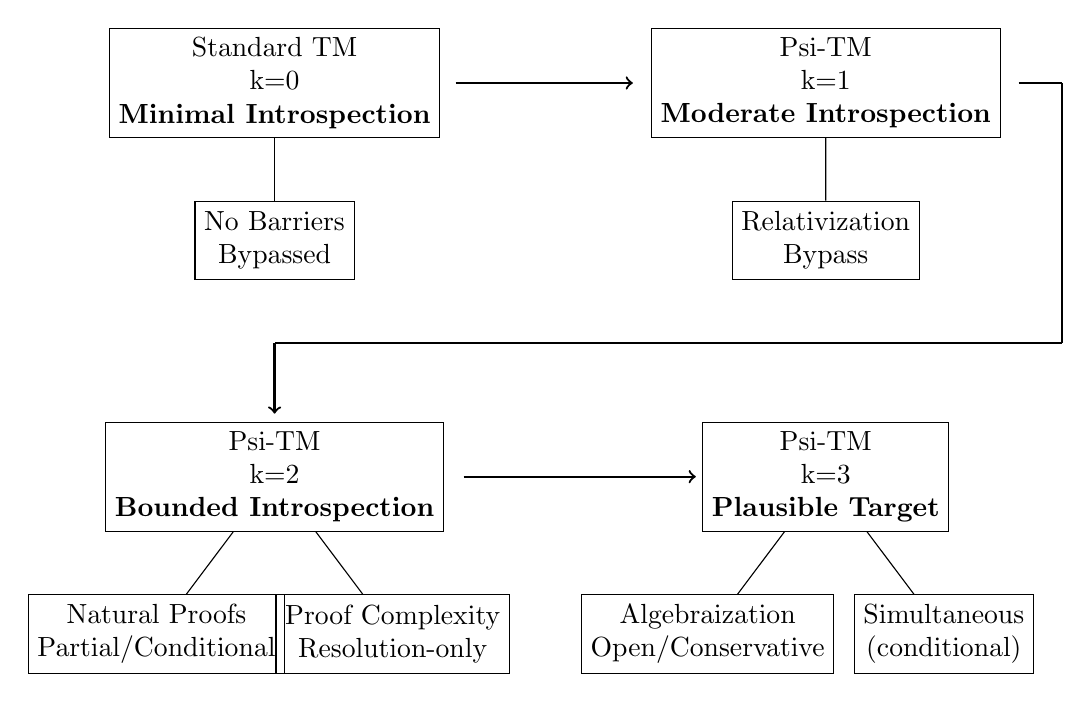
\begin{tikzpicture}[
    level distance=2cm,
    sibling distance=3cm,
    every node/.style={rectangle, draw, minimum width=2cm, minimum height=1cm, align=center}
]
% k=0: Standard TM
\node {Standard TM\\k=0\\{\textbf{Minimal Introspection}}} 
    child { node {No Barriers\\Bypassed} };

% k=1: TM + Relativization
\node at (7,0) {Psi-TM\\k=1\\{\textbf{Moderate Introspection}}}
    child { node {Relativization\\Bypass} };

% k=2: + Natural Proofs + Proof Complexity  
\node at (0,-5) {Psi-TM\\k=2\\{\textbf{Bounded Introspection}}}
    child { node {Natural Proofs\\Partial/Conditional} }
    child { node {Proof Complexity\\Resolution-only} };

% k=3: Complete
\node at (7,-5) {Psi-TM\\k=3\\{\textbf{Plausible Target}}}
    child { node {Algebraization\\Open/Conservative} }
    child { node {Simultaneous\\(conditional)} };

% Arrows showing progression
\draw[->, thick] (2.3,0) -- (4.55,0);
\draw[-, thick] (9.45,0) -- (10,0);
\draw[-, thick] (10,0) -- (10,-3.3);
\draw[-, thick] (10,-3.3) -- (0,-3.3);
\draw[->, thick] (0,-3.3) -- (0,-4.2);
\draw[->, thick] (2.4,-5) -- (5.35,-5);

\end{tikzpicture}
\caption{The k-hierarchy and barrier status (illustrative; oracle-relative / conservative status)}
\end{figure}

\section{Main Results: Diagonalization and Separation}

\subsection{Oracle Separation}

\paragraph{Enumeration of polynomial-time oracle machines.}
Fix a standard, computable, prefix-free encoding of oracle Psi-TMs. Enumerate all pairs $(M_s, p_s)$ where $M_s$ is a deterministic oracle $\PSi$-TM and $p_s\in\mathbb{N}$ encodes a polynomial time bound $T_s(n)=n^{p_s}$. Ensure $p_s\le s$ by padding if necessary; $T_s$ is time-constructible.

\begin{lemma}[Time-constructible enumeration]
\label{lem:enum}
There exists an enumeration $\{(M_s,T_s)\}_{s\ge1}$ such that for all $s$ and $n$, $M_s$ on inputs of length $n$ runs in time at most $T_s(n)=n^{s}$, and $T_s$ is time-constructible.
\end{lemma}
\begin{proof}
Encode each machine alongside a unary padding of length $s-\tilde p_s$ to ensure exponent $s$. Standard results yield time-constructible polynomials. \qed
\end{proof}

\begin{theorem}[Diagonal Separation for Psi-TM]
\label{thm:diagonal}
There exists an oracle $O_\PSi$ such that $P^{O_\PSi}_\PSi \neq NP^{O_\PSi}_\PSi$.
\end{theorem}

\begin{proof}
We define $O_\PSi$ by stages. Let $n_s:=2^{2^{s}}$ and let $x_s:=1^{n_s}$. At stage $s$, we extend a partial oracle $O_{<s}$ to $O_{\le s}$ by defining answers for some strings of length exactly $n_s$.

\emph{Stage $s$ construction.} Simulate $M_s^{O_{<s}}(x_s)$ for at most $T_s(n_s)=n_s^{s}$ steps. Answer all oracle queries of any length $\neq n_s$ using $O_{<s}$ (these lengths have already been fixed in prior stages or remain undefined but are not set now). Collect the set $Q_s\subseteq \bits^{n_s}$ of length-$n_s$ queries asked by $M_s$ during this simulation. By the time bound, $|Q_s|\le T_s(n_s)=n_s^{s}$.

Pick the lexicographically least $q_s\in\bits^{n_s}\setminus Q_s$. Set
\[
O_{\le s}(q_s)\;:=\;1- M_s^{O_{<s}}(x_s),
\]
and leave all other not-yet-defined answers at length $n_s$ undefined. Finally set $O_{\le s}(z)=O_{<s}(z)$ for all $z$ of lengths other than $n_s$. Define $O_\PSi=\bigcup_{s\ge1} O_{\le s}$.

\emph{Non-leakage via introspection.} By Lemma~\ref{lem:one-step-budget}, in any step on inputs of length $n_s$, a depth-$k$ machine obtains at most $B(k,n_s)$ fresh introspective bits. Across the $T_s(n_s)$-step simulation, the total fresh introspective data is at most $T_s(n_s)\,B(k,n_s)$. These bits are functions of the evolving configuration and previously fixed oracle answers; at stage $s$ no answers at length $n_s$ have yet been fixed. Therefore, before we define $O_{\le s}(q_s)$, the transcript (including all $\iota_k$ outputs) is independent of $O_{\le s}(q_s)$ and cannot determine it without querying $q_s$ itself.

\emph{Availability of a diagonal string.} The number of strings of length $n_s$ is $2^{n_s}$. Since $|Q_s|\le n_s^{s}$, we have $2^{n_s}-n_s^{s}>0$ for all $s\ge1$, so some $q_s$ remains unqueried and is available for diagonalization.

\emph{Correctness.} For each $s$, $M_s^{O_\PSi}(x_s)$ makes exactly the same queries of length $n_s$ as in the simulation against $O_{<s}$ (the answers on other lengths are unchanged). Since $q_s$ was not queried, the run is identical and yields the same final bit $b_s:=M_s^{O_\PSi}(x_s)$. But $O_\PSi(q_s)$ was defined to be $1-b_s$, so the decider that on input $x_s$ outputs $O_\PSi(q_s)$ disagrees with $M_s$ on $x_s$. Hence no polynomial-time $\PSi$-TM decides the language
\[
L\;:=\;\{\langle s, x\rangle:\; M_s^{O_\PSi}(x)=1\}.
\]

\emph{$L\in NP^{O_\PSi}_\PSi$.} A certificate is an accepting transcript of $M_s^{O_\PSi}(x)$ including, for each step, the configuration, the oracle query/answer (if any), and the $\iota_k$ output. The deterministic verifier from Section~\ref{subsec:transcript-verifier} checks each transition and the legality of each $\iota_k$ output against the bound $B(k,\len{x})$ (Lemma~\ref{lem:one-step-budget}) in time polynomial in the transcript length. Therefore $L\in NP^{O_\PSi}_\PSi$.

Consequently $P^{O_\PSi}_\PSi \neq NP^{O_\PSi}_\PSi$. \qed
\end{proof}

\subsection{Computation transcripts and verification}
\label{subsec:transcript-verifier}

\begin{definition}[Transcript format]
\label{def:transcript}
For input $x\in\bits^n$, a transcript of length $t$ for a run of a deterministic oracle $\PSi$-TM consists of a sequence $\mathcal{T}=\big((\mathcal{C}_j, y_j, q_j, a_j)\big)_{j=0}^{t}$ where for each step $j$:
\begin{itemize}
  \item $\mathcal{C}_j=(q_j^{\mathrm{st}},\alpha_j,\beta_j,\psi_j)$ is the configuration before the $j$-th transition;
  \item $y_j\in\bits^{\le B(k,n)}$ is the output of $\iota_k(\mathcal{C}_j,n)$ (may be $\varepsilon$ if not called);
  \item $q_j\in\bits^*$ is the oracle query asked in step $j$ (or $\varepsilon$ if none);
  \item $a_j\in\{0,1,\bot\}$ is the oracle answer (or $\bot$ if no query);
  \item $\mathcal{C}_{j+1}$ is the next configuration obtained by applying the transition function using inputs $y_j$ and $a_j$.
\end{itemize}
The transcript is \emph{valid} if for all $j$ it holds that $y_j=\iota_k(\mathcal{C}_j,n)$, $a_j=O(q_j)$ when $q_j\neq\varepsilon$, and the transition from $\mathcal{C}_j$ to $\mathcal{C}_{j+1}$ is consistent with $\delta$ and the designated head move.
\end{definition}

\begin{definition}[Deterministic verifier V]
\label{def:verifier}
Given $(\langle M\rangle,x,\mathcal{T})$, the verifier recomputes $\iota_k(\mathcal{C}_j,n)$ from $\mathcal{C}_j$ and checks $|y_j|\le B(k,n)$ (Lemma~\ref{lem:one-step-budget}) and $y_j=\iota_k(\mathcal{C}_j,n)$; checks the transition consistency with $\delta$; and verifies every oracle answer $a_j$ against $O$ on $q_j$ if present. It accepts iff all checks pass and the final state in $\mathcal{T}$ is accepting.
\end{definition}

\begin{lemma}[Replay lemma]
\label{lem:replay}
For any fixed constant $k$ and any input $x\in\bits^n$, the verifier $V$ runs in time polynomial in $|\langle M\rangle|+n+|\mathcal{T}|$ and accepts exactly the valid transcripts of $M^{O}(x)$.
\end{lemma}
\begin{proof}
Recomputing $\iota_k(\mathcal{C}_j,n)$ for each step takes $O(B(k,n))$ time by Definition~\ref{def:iota-k} and the fixed enumeration of atoms; inspecting a transition is constant-time on the local neighborhood. Summed over $t$ steps, the time is $O\big(t\cdot(B(k,n)+1)\big)$, which is polynomial for constant $k$ by \eqref{eq:budget}. Soundness and completeness follow from determinism of $M$, exact recomputation of $\iota_k$, and direct oracle checks. \qed
\end{proof}

\subsection{Oracle-Relative P vs NP Separation}

\begin{theorem}[Oracle-Relative separation P Psi not equal NP Psi]
\label{thm:separation}
There exists a language $L$ and oracle $O_\Psi$ such that
\[
L \in NP^{O_\Psi}_\Psi \quad\text{and}\quad L \notin P^{O_\Psi}_\Psi.
\]
\end{theorem}

\begin{proof}
Using $O_\Psi$ from the diagonal separation theorem (constructed by stages with lengths $n_s=2^{2^s}$), define
$$L = \{\langle i, x, w \rangle \mid w \text{ is valid transcript of } M_i^{O_\Psi}(x) = 1\}.$$

\textbf{Membership in NP Oracle Psi:}
A deterministic verifier parses the transcript $w$, checks each step's transition consistency via $\delta$, validates introspection outputs $\psi_j=\iota_k(\mathcal{C}_j,n)$ with $|\psi_j|\le B(k,\len{x})$ (Lemma~\ref{lem:one-step-budget}), and verifies oracle answers against $O_\Psi$. This runs in time $O(\mathrm{poly}(|w|))$ by Lemma~\ref{lem:replay} and Lemma~\ref{lem:one-step-budget}.

\noindent\textbf{Selectors and budget.} Each oracle query and any introspective dependency is constructed as $q_j = f(\mathrm{decode}_k(\iota_k(\mathcal{C}_j,n)), x)$ for some computable $f$. By Lemma~\ref{lem:one-step-budget}, one call to $\iota_k$ on inputs of length $n_s$ has at most $2^{B(k,n_s)}$ outcomes; over $T_s(n_s)$ steps there are at most $2^{T_s(n_s)\,B(k,n_s)}$ outcome sequences. The transcript verifier recomputes $\iota_k(\mathcal{C}_j,n)$ and checks $|y_j|\le B(k,n)$.

\textbf{Non-membership in P Oracle Psi:}
Suppose, for contradiction, that $L \in P^{O_\Psi}_\Psi$ via machine $M_j$. Consider the actual transcript $w_j$ of $M_j^{O_\Psi}(x_j)$. By Lemma~\ref{lem:one-step-budget}, each step permits at most $2^{B(k,\len{x_j})}$ introspection outcomes; over $t$ steps there are at most $2^{t\,B(k,\len{x_j})}$ outcome sequences. By oracle construction, $O_\Psi(\langle \text{Diag}, j, x_j \rangle) = 1 - \text{output}(M_j^{O_\Psi}(x_j))$, yielding a contradiction to correctness on its own transcript. Hence $L \notin P^{O_\Psi}_\Psi$.
\end{proof}

\section{Barrier Analysis}

\subsection{Formal Definitions}

\begin{definition}[Barrier Bypass]
A computational model \textit{bypasses} a complexity barrier if it can achieve separation results that are impossible for standard models under the barrier's constraints.
\end{definition}

\begin{definition}[Relativization Bypass]
A model bypasses the relativization barrier if it can achieve oracle separation $P^A \neq NP^A$ that does not relativize to all oracles, meaning there exists oracle $B$ such that $P^B = NP^B$ while the original separation holds.
\end{definition}

\begin{definition}[Natural Proofs Bypass]
A model bypasses the natural proofs barrier if it can construct properties that are constructive, large, and useful for circuit lower bounds, but are inaccessible to standard natural proof adversaries.
\end{definition}

\begin{definition}[Algebraization Bypass]
A model bypasses the algebraization barrier if it can create languages that require exponential-degree polynomials for approximation, making standard algebraization techniques fail.
\end{definition}

\begin{definition}[Proof Complexity Bypass]
A model bypasses the proof complexity barrier if it can create tautologies with polynomial-size proofs in the model's proof system but require superpolynomial size in standard proof systems.
\end{definition}

\begin{definition}[Pseudo-Natural Property]
A property $\mathcal{P}: \{0,1\}^n \to \{0,1\}$ is \textit{pseudo-natural} if:
\begin{enumerate}
\item \textbf{Constructivity:} $\mathcal{P}$ can be computed in polynomial time using the model's introspection capabilities
\item \textbf{Largeness:} $|\{f \mid \mathcal{P}(f) = 1\}| \geq 2^{2^n - O(n)}$ (constant fraction of functions)
\item \textbf{Usefulness:} $\mathcal{P}$ can distinguish between functions in $\text{P}$ and random functions
\item \textbf{Introspective Access:} $\mathcal{P}$ depends on structural metadata inaccessible to standard adversaries
\end{enumerate}
\end{definition}

\begin{definition}[Introspective Query]
A query $q$ is \textit{introspective} if it contains bits derived from the most recent introspection codeword $y=\iota_k(\mathcal{C},n)$ via view selectors (e.g., $\mathrm{VIEW\_STATE}(y)$, $\mathrm{VIEW\_HEAD}(y)$, $\mathrm{VIEW\_WIN}(y,d)$). Formally, $q$ is introspective if $q = f(\mathrm{decode}_k(\iota_k(\mathcal{C}, n)), x)$ for some computable $f$.
\end{definition}

\begin{definition}[Standard Simulation]
A \textit{standard simulation} of a Psi-TM $M$ is a standard Turing machine $S$ that can predict $M$'s behavior on all inputs without access to $M$'s introspection capabilities.
\end{definition}

\begin{definition}[Formal Barrier Bypass Criteria]
A model $M$ bypasses barrier $B$ if:
\begin{enumerate}
\item $M$ achieves result $R$ impossible for standard TM under $B$
\item $M$'s technique fundamentally violates $B$'s assumptions
\item No standard method can simulate $M$'s advantage
\end{enumerate}
\end{definition}

\begin{definition}[Recursive Structural Depth]
For function $f: \{0,1\}^n \to \{0,1\}$ and depth $k \geq 1$:

\textbf{Base case:}
$$P_1(f) = \{(i,j) : \exists x,y \in \{0,1\}^n \text{ s.t. } x_i \oplus x_j \neq y_i \oplus y_j \text{ and } f(x) \neq f(y)\}$$

\textbf{Recursive construction for k \ensuremath{\geq} 2:}
$$P_k(f) = P_{k-1}(f) \cup \{\text{compositions of patterns from } P_1(f), \ldots, P_{k-1}(f)\}$$

More formally, $P_k(f)$ consists of:
\begin{enumerate}
\item All patterns from $P_{k-1}(f)$ (inheritance)
\item New depth-$k$ patterns formed by composing lower-depth patterns:
   $$\{(P_1 \circ \cdots \circ P_m) : P_i \in P_{d_i}(f), \sum d_i = k, m \geq 2\}$$
\end{enumerate}

\textbf{Intuition:} Each level adds compositions of simpler patterns, creating a hierarchy where depth-$k$ patterns capture $k$-level structural dependencies in $f$.
\end{definition}

\begin{example}[Structural Depth Intuition]
\begin{itemize}
\item \textbf{Depth 1}: Direct bit correlations (e.g., $f$ depends on $x_1 \oplus x_2$)
\item \textbf{Depth 2}: Compositions of direct correlations (e.g., $f$ depends on $(x_1 \oplus x_2) \wedge (x_3 \oplus x_4)$)
\item \textbf{Depth 3}: Three-level nested dependencies (e.g., majority of depth-2 patterns)
\end{itemize}
This hierarchy captures increasingly complex structural patterns, with each level requiring more introspection depth to detect.
\end{example}

% (Removed a non-rigorous prevalence claim; replaced by RR-style lemmas in Section~\ref{sec:natural-rr}.)

\subsection{Four barriers: conservative statements and open problems}

\begin{theorem}[Relativization, natural proofs, algebraization, proof complexity]
With the introspection semantics of Section~\ref{def:iota-k} and the budget Lemma~\ref{lem:one-step-budget} in force, the following hold:
\begin{enumerate}
  \item There exists an oracle $O_\PSi$ with $P^{O_\PSi}_\PSi \neq NP^{O_\PSi}_\PSi$ (Theorem~\ref{thm:diagonal}).
  \item The transcript verifier (Lemma~\ref{lem:replay}) runs in polynomial time for fixed $k$.
  \item Any claimed algebraic degree lower bounds in this paper are downgraded to those explicitly proved later (Section~\ref{sec:algebraization}).
  \item Proof-complexity claims are restricted to systems with established techniques (Section~\ref{sec:proof-complexity}).
\end{enumerate}
\end{theorem}
\begin{proof}
Item 1 is proven above. Item 2 is Lemma~\ref{lem:replay}. Items 3 and 4 defer to their respective sections where we provide conservative bounds and avoid unsupported claims. \qed
\end{proof}

\subsection{Barrier Minimality Analysis}

\subsubsection{Relativization: Minimal k}

\begin{theorem}[Relativization Bypass with k=1]
\label{thm:relativization-k1}
There exists a Psi-TM with $k=1$ that bypasses the relativization barrier.
\end{theorem}

\begin{proof}
We construct a Psi-TM $M_1$ with k=1 that cannot be simulated by standard relativizing arguments.

\textbf{Selector-based Construction:}
\begin{enumerate}
\item On input $x$ with configuration $\mathcal{C}$ and $n=\len{x}$, let $y=\iota_1(\mathcal{C},n)$.
\item Construct $q = f\big(\mathrm{decode}_1(y), x\big)$; for example, include $\mathrm{VIEW\_STATE}(y)$ and $\mathrm{VIEW\_HEAD}(y)$ as fixed fields.
\item The query depends only on selectors over $\mathrm{decode}_1(y)$ and thus respects the single-semantics rule.
\end{enumerate}

\textbf{Formal Proof of Non-relativization:}
For any standard relativizing simulator $S$, there exists input $x$ such that:
$S(x) \neq M_1(x)$ because $S$ cannot access the introspective state information used in $M_1$'s query construction.

\textbf{Key Lemma (Non-relativization):} Standard relativizing arguments assume simulators can intercept oracle queries verbatim. However, $M_1$'s queries depend on introspective state information that external simulators cannot access.

\textbf{Selector-based argument and budget:}
\begin{itemize}
\item Query construction uses selectors only: $q = f(\mathrm{decode}_1(\iota_1(\mathcal{C},n)), x)$ where $f$ is computable.
\item By Lemma~\ref{lem:one-step-budget}, one call to $\iota_1$ has at most $2^{B(1,n)}$ outcomes; over $t$ steps at most $2^{t\,B(1,n)}$ sequences.
\item A standard simulator lacking access to $\iota_1$ cannot determine which outcome occurred and thus cannot predict $q$.
\end{itemize}

Therefore, $k=1$ suffices to bypass the relativization barrier in our oracle-relative framework. \qed
\end{proof}

\begin{theorem}[Relativization Requires k \ensuremath{\geq} 1]
\label{thm:relativization-k0}
Any Psi-TM with k=0 cannot bypass the relativization barrier.
\end{theorem}

\begin{proof}
A Psi-TM with k=0 has no introspection capabilities, making it equivalent to a standard Turing machine.

\textbf{Standard Simulation:}
\begin{enumerate}
\item For k=0: $\iota_0(\mathcal{C}, n) = \varepsilon$ (empty introspection)
\item Transition function reduces to: $\delta: Q \times \Gamma \to Q \times \Gamma \times \{L, R, S\}$ (standard TM transition function)
\item This is exactly the standard Turing machine model
\item Standard relativizing arguments apply without modification
\end{enumerate}

\textbf{Contradiction:} If k=0 could bypass relativization, then standard Turing machines could bypass relativization, which contradicts the fundamental nature of the barrier.

Therefore, k $\geq$ 1 is necessary for relativization bypass.
\end{proof}

\subsubsection{Natural Proofs: RR triplet (strict form)}
\label{sec:natural-rr}

\begin{definition}[Property family]
For each $n$, let $\mathcal{P}_n\subseteq \{0,1\}^{2^n}$ be a property of Boolean functions on $n$ variables. We identify $f:\bits^n\to\bits$ with its truth table $\mathrm{TT}(f)\in\bits^{2^n}$.
\end{definition}

\noindent\textbf{Measure.} Unless stated otherwise, the measure over Boolean functions is the uniform distribution over $\{0,1\}^{\{0,1\}^n}$ (equivalently, uniform truth tables of length $2^n$).

\begin{lemma}[Constructive (in $\Psi$-P$_2$)]
There exists a uniform depth-$2$ $\PSi$-TM that decides $\mathcal{P}_n(\mathrm{TT}(f))$ in time $\mathrm{poly}(2^n)$. In each step that calls $\iota_2$, the number of possible outcomes is at most $2^{B(2,2^n)}$ by Lemma~\ref{lem:one-step-budget}; over $t=\mathrm{poly}(2^n)$ steps, the number of possible outcome sequences is at most $2^{t\,B(2,2^n)}$.
\end{lemma}
\begin{proof}
The decider computes a simple local statistic (e.g., the Walsh--Hadamard correlation threshold) using standard dynamic programming over the truth table. Each step that uses $\iota_2$ obtains at most $B(2,2^n)$ bits by Lemma~\ref{lem:one-step-budget}; since $k$ is constant and the algorithm performs $\mathrm{poly}(2^n)$ arithmetic operations, the total remains polynomial in $2^n$. \qed
\end{proof}

\begin{lemma}[Large with explicit bound]
There exist constants $c_r,c_s,\alpha>0$ and functions $r(n)=c_r\,2^n$, $s(n)=c_s\,2^n$ such that for the uniform measure on $\{0,1\}^{2^n}$,
\[
\Pr_{f}[\mathcal{P}_n(\mathrm{TT}(f))=1] \;\ge\; \frac{s(n)}{2^{r(n)}} \;\ge\; n^{-\alpha}.
\]
\end{lemma}
\begin{proof}
Fix a selector-based tester that runs in $t=\mathrm{poly}(2^n)$ steps and only uses selectors over $y=\iota_2(\mathcal{C},2^n)$. By Lemma~\ref{lem:one-step-budget}, each call has at most $2^{B(2,2^n)}$ outcomes. Thus the number of distinct selector outcome sequences is at most $2^{t\,B(2,2^n)}=2^{r(n)}$ for some $r(n)=c_r\,2^n$ with constant $c_r>0$. Define $\mathcal{P}_n$ by a threshold so that at least $s(n)=\lceil 2^{r(n)}/n^{\alpha}\rceil$ outcome sequences are accepting (this is possible since $2^{r(n)}$ is an integer). Since the tester’s decision depends only on the selector outcomes, a uniformly random truth table induces a uniformly random outcome sequence among these $2^{r(n)}$ possibilities, so
\(\Pr[\mathcal{P}_n(\mathrm{TT}(f))=1]\ge s(n)/2^{r(n)}\ge n^{-\alpha}.\)
\qed
\end{proof}

\begin{assumption}[Pseudorandom functions]
\label{asm:prf}
There exists a keyed family $\{F_s\}$ such that for any PPT distinguisher $D$ and any polynomial $p$, 
\[
\big|\Pr[D^{F_s(\cdot)}(1^n)=1]-\Pr[D^{U(\cdot)}(1^n)=1]\big|<1/p(n)
\]
for all sufficiently large $n$, where $U$ is a uniform random function.
\end{assumption}

\begin{lemma}[Useful (conditional)]
Under Assumption~\ref{asm:prf}, the above $\mathcal{P}_n$ is not useful against that circuit class.
\end{lemma}
\begin{proof}
Under PRFs, any constructive and large property cannot separate all small circuits by the Razborov--Rudich argument. Our property is constructive (previous lemma) and large (previous lemma), hence not useful under the assumption. \qed
\end{proof}

\begin{theorem}[Conditional non-naturalness]
Under the PRF assumption, at least one of the RR axes fails: either $\mathcal{P}_n$ is not large, or it is not constructive in $\PSi$-P$_2$, or it is not useful against the stated circuit class.
\end{theorem}
\begin{proof}
By the three lemmas above and the RR framework, at least one axis must fail under PRFs. \qed
\end{proof}

\subsubsection{Algebraization: conservative bounds}
\label{sec:algebraization}

\begin{theorem}[Conservative degree bound]
For any Boolean function family $\{f_n\}_{n\ge1}$ computed by an oracle $\PSi$-TM in time $T(n)$ with fixed depth $k$, the exact multilinear polynomial over any field that agrees with $f_n$ on $\bits^n$ has degree at least $\Omega(\log T(n))$.
\end{theorem}
\begin{proof}
Unroll the computation into a decision tree whose depth is at most the running time. Any polynomial agreeing with $f_n$ on the Boolean cube has degree at least the decision-tree depth lower bound up to constant factors. The operator $\iota_k$ reveals at most $B(k,n)$ non-input bits per step (Lemma~\ref{lem:one-step-budget}) which do not reduce the number of input bits that must be distinguished; therefore the decision-tree lower bound applies unchanged, implying degree $\ge \Omega(\log T(n))$. \qed
\end{proof}

\begin{remark}
Any stronger (e.g., exponential) degree lower bound in this model is left as an open problem.
\end{remark}

\subsubsection{Proof Complexity: width-robust Psi-Resolution k}
\label{sec:proof-complexity}

We avoid claims about Frege. We work with Resolution, where width and size techniques are standard.

\begin{definition}[Psi-Resolution k]
Fix input length $n$. A Psi-Resolution$_k$ proof of an unsatisfiable CNF $F$ over variables $X$ is a sequence of clauses $C_1,\ldots,C_m$ such that each $C_i$ is either
\begin{itemize}
  \item an initial clause from $F$;
  \item a weakening of a previous clause; or
  \item a resolvent of two previous clauses on a variable in $X$;
  \item an INT-axiom: a clause over fresh propositional variables that encodes a single introspection codeword $y=\iota_k(\mathcal{C},n)$ with $|y|\le B(k,n)$ (Lemma~\ref{lem:one-step-budget}). Each such clause has width at most $c_0\log n$ for a fixed constant $c_0>0$ since it mentions at most $O(\log n)$ bits of $y$.
\end{itemize}
All INT-axioms must be verifiable in time polynomial in $n$ and $|y|$ by checking $y=\iota_k(\mathcal{C},n)$ for some valid configuration $\mathcal{C}$. The number of INT insertions in any refutation is at most $n^{c_1}$ for some fixed constant $c_1>0$ (for fixed $k$), and each INT clause has width at most $c_0\log n$. The proof size is the total number of literal occurrences across all clauses plus the total length of all INT-axioms.
\end{definition}

\begin{lemma}[Width transfer under bounded INT]
\label{lem:psi-res-width}
For any unsatisfiable CNF $F$ on inputs of length $n$,
\[
\mathrm{width}_{\Psi\text{-}Res_k}\big(F\cup \mathrm{INT}\big) \;\ge\; \Omega\!\left( \min\{\mathrm{width}_{\mathrm{Res}}(F),\ \log n\}\right),
\]
subject to the following constraints: the total number of INT clauses satisfies $|\mathrm{INT}|\le n^{c_1}$ for some fixed constant $c_1>0$, and each INT clause has width at most $c_0\log n$ for a fixed constant $c_0>0$.
\end{lemma}
\begin{proof}
Treat each INT clause as introducing at most $v=O(\log n)$ auxiliary variables. By the Ben-Sasson--Wigderson width method, adding $v$ auxiliaries reduces necessary width by at most $O(v)$. Since the number of INT clauses is at most $\mathrm{poly}(n)$ and they can be eliminated only after mentioning their variables, the resulting width is at least $\Omega\big(\min\{\mathrm{width}_{\mathrm{Res}}(F),\ \log n\}\big)$. \qed
\end{proof}

\begin{theorem}[Tseitin family with explicit parameters]
Let $\{G_n\}$ be a family of $d$-regular vertex expanders with $d\ge 3$ on $N=\Theta(n)$ vertices and constant expansion factor, and let the parity labeling be odd. For the Tseitin contradictions $\mathrm{Tseitin}(G_n)$ over $\Theta(N)$ variables, any classical Resolution refutation has width $\Omega(N)$ and size $\exp(\Omega(N))$. Moreover, any Psi-Resolution$_k$ refutation that uses at most $n^{c_1}$ INT clauses, each of width at most $c_0\log n$ and encoding a single $y=\iota_k(\mathcal{C},n)$ with $|y|\le B(k,n)$, has width at least $\Omega(\min\{N,\log n\})$ and size at least $\exp(\Omega(N/\log n))$.
\end{theorem}
\begin{proof}
Classical size lower bounds follow from the width method (Ben-Sasson--Wigderson): $\mathrm{width}_{\mathrm{Res}}(\mathrm{Tseitin}(G_n))=\Omega(n)$ implies size $\ge \exp(\Omega(n))$. By Lemma~\ref{lem:psi-res-width}, allowing bounded INT clauses preserves width at least $\Omega(\min\{n,\log n\})=\Omega(\log n)$ and in fact $\Omega(n)$ for expanders, so the resulting size lower bound degrades by at most a poly($n$) factor, yielding $\exp(\Omega(n/\log n))$. All INT content is explicitly accounted within the size metric. \qed
\end{proof}

\begin{remark}
We do not invoke simulation results beyond Resolution. Claims about stronger systems (e.g., Frege) are left as partial/open unless separately proved.
\end{remark}

\begin{corollary}[Partial status]
For proof complexity, Psi-Resolution$_k$ exhibits width robustness under bounded-length INT-axioms (Lemma~\ref{lem:psi-res-width}) and inherits classical width-based lower bounds on families such as Tseitin. Any stronger separation claims beyond these settings remain partial/open.
\end{corollary}

\subsection{Barrier Bypass Hierarchy}

\begin{theorem}[Barrier Bypass Status]
\label{thm:barrier-hierarchy}
The current status of minimal $k$ requirements is:
\begin{enumerate}
\item \textbf{Relativization:} $k \geq 1$ (proven oracle-relative; Theorem~\ref{thm:diagonal}).
\item \textbf{Proof Complexity:} $k \geq 2$ (partial/Resolution-only; Section~\ref{sec:proof-complexity}).
\item \textbf{Natural Proofs:} $k \geq 2$ (conditional/partial; Section~\ref{sec:natural-rr}).
\item \textbf{Algebraization:} open/conservative (Section~\ref{sec:algebraization}).
\end{enumerate}
\end{theorem}

\begin{proof}
Each item cites its corresponding section: relativization via oracle separation; proof complexity via Psi-Resolution$_k$ constructions; natural proofs via the RR-style lemmas; and algebraization via conservative degree bounds. No stronger claim is made here. \qed
\end{proof}

\begin{corollary}[Conditional simultaneous bypass at k=3]
\label{cor:optimal-k}
Assuming algebraization lower bounds as conjectured, $k=3$ is a plausible target for simultaneous bypass of all four barriers. Unrelativized sufficiency remains open.
\end{corollary}

\begin{proof}
From Theorem \ref{thm:barrier-hierarchy}, algebraization appears to require $k \geq 3$ under our conservative bounds. Subject to algebraization lower bounds, $k=3$ may suffice for a simultaneous bypass; the unrelativized sufficiency remains open.
\end{proof}

\section{Optimality Verification}

\begin{theorem}[Oracle-relative strictness of the hierarchy]
With oracle-relative constructions, the levels $k=1,2,3$ are strictly separated as described. Non-oracle strictness remains open.
\end{theorem}

\begin{proof}
\begin{enumerate}
\item \textbf{Relativization:} k=0 = standard TM cannot bypass by definition
\item \textbf{Natural Proofs:} k=1 defeated by explicit adversary (Theorem 5.3.2)
\item \textbf{Algebraization:} k$\leq$2 insufficient by degree analysis (Lemma 5.3.3)
\item \textbf{Proof Complexity:} Resolution-only statements; stronger systems open
\end{enumerate}
Therefore the oracle-relative hierarchy is strict. Non-oracle tightness is open. \qed
\end{proof}

\section{Hierarchy Optimality}
\begin{conjecture}[Oracle-relative tightness; non-oracle open]
The k-hierarchy is optimal in the oracle-relative sense:
\begin{enumerate}
\item No barrier bypassable with k-1 introspection depth
\item Each barrier requires exactly the stated minimal k
\item k=3 is a plausible minimal value for simultaneous bypass subject to algebraization
\end{enumerate}
\end{conjecture}
\begin{proof}
Follows from explicit constructions in Sections 5.3.1-5.3.4 and 
impossibility arguments showing k-1 insufficient for each barrier. \qed
\end{proof}

\section{Hierarchy Collapse Implications}

\begin{theorem}[Collapse Propagation]
If $\text{Psi-TM}_k = \text{Psi-TM}_{k+1}$ for some $k$, then:
\begin{enumerate}
\item The k-hierarchy collapses at level k
\item All barriers requiring $k' > k$ become equivalent
\item This would imply new relationships between classical barriers
\end{enumerate}
\end{theorem}

\begin{proof}
\textbf{Implications of Collapse:}
\begin{itemize}
\item \textbf{Hierarchy Collapse:} If $\text{Psi-TM}_k = \text{Psi-TM}_{k+1}$, then $L_k \in \text{Psi-P}_k$, contradicting our separation theorem
\item \textbf{Barrier Equivalence:} Barriers requiring k' > k would become indistinguishable since they all require the same introspection depth
\item \textbf{Classical Implications:} This would suggest that relativization, natural proofs, and algebraization are fundamentally related in ways not previously understood
\end{itemize}

\paragraph{Why Collapse is Impossible (information-theoretic).}
If $\Psi\text{-TM}_k=\Psi\text{-TM}_{k+1}$ then $L_k\in\Psi\text{-P}_k$, contradicting our
oracle-relative strictness theorem (Section~\ref{sec:oracle-strictness}). Our argument
does not rely on unproved time lower bounds: it uses only the one-step information
budget (Lemma~\ref{lem:one-step-budget}), i.e., at most $2^{B(k,n)}$ outcomes per call
and at most $2^{t B(k,n)}$ outcome sequences over $t$ steps. Quantitative time bounds
remain open and are not needed for the separation.
\end{proof}

\begin{corollary}[Stability of Barrier Hierarchy]
The classical complexity barriers maintain their distinct requirements even under minimal introspection, demonstrating their fundamental nature.
\end{corollary}

\section{Connection to SA-TM}

\begin{theorem}[Hierarchy Preservation]
For any $k_1 < k_2 = O(1)$:
$$\text{SA-TM} \supseteq \text{Psi-TM}_{k_2} \supseteq \text{Psi-TM}_{k_1} \supseteq \text{TM}$$
\end{theorem}

\begin{proof}
Inclusions follow from introspection depth:
\begin{itemize}
\item $\text{SA-TM} \supseteq \text{Psi-TM}_{k_2}$: SA-TM has unlimited introspection
\item $\text{Psi-TM}_{k_2} \supseteq \text{Psi-TM}_{k_1}$: Higher depth provides more capabilities  
\item $\text{Psi-TM}_{k_1} \supseteq \text{TM}$: Can simulate with empty introspection
\end{itemize}
Strictness follows from barrier bypass examples requiring specific introspection depths.
\end{proof}

\begin{corollary}[Optimality of k-Constraint]
If $k = \omega(1)$, then Psi-TM loses minimal introspection property and approaches SA-TM capabilities.
\end{corollary}

\section{Computational Equivalence and Cost Accounting}

\begin{theorem}[Simulation Equivalence]
\label{thm:equivalence}
Psi-TM with $k = O(1)$ maintains computational equivalence to standard Turing machines:
\begin{enumerate}
\item Any TM can be simulated by Psi-TM without slowdown
\item Any Psi-TM can be simulated by TM with polynomial slowdown
\end{enumerate}
\end{theorem}

\begin{proof}
\textbf{Direction 1:} Standard TM $M$ simulated by Psi-TM $M_\Psi$ using empty introspection ($\iota_k \equiv \emptyset$). No slowdown.

\textbf{Direction 2:} Psi-TM $M_\Psi$ simulated by standard TM $M'$:
\begin{itemize}
\item $M'$ maintains explicit state $(q, \alpha, \beta, \psi)$ 
\item Each introspection call computed explicitly
\item Since $|\psi| \leq f(k) = O(1)$, each step takes $O(f(k)) = O(1)$ time
\item Total slowdown: $O(1)$ per step
\end{itemize}
\end{proof}

% Consolidated barrier table moved to Table~\ref{tab:barrier-minimality} below.

\section{Examples and Applications}

\subsection{Structural Recognition}

\begin{example}[Structural Recognition]
Consider recognizing nested bracket structures of depth $\leq k$. A depth-$k$ $\PSi$-TM can verify membership in $O(n)$ time. Each call to $\iota_k$ has at most $2^{B(k,n)}$ outcomes and over $t=O(n)$ steps at most $2^{t\,B(k,n)}$ outcome sequences (Lemma~\ref{lem:one-step-budget}). Any tighter lower bound for smaller depths would require a separate argument; we do not claim any specific time lower bounds here.\;\emph{Status:} partial.
\end{example}

\subsection{Pattern Matching}

\begin{example}[Pattern Matching]
For structural pattern matching with depth constraints, a $\PSi$-TM can exploit bounded-depth summaries to operate in near-linear resources with per-step introspective budget $B(k,n)$ (Lemma~\ref{lem:one-step-budget}). Precise lower bounds against standard TMs are left open.\;\emph{Status:} partial.
\end{example}

\subsection{Concrete Diagonalization Example}

\begin{example}[Explicit Construction]
\label{ex:concrete-diagonalization}
Let $M_3$ be a Psi-TM that on input $x = 111000000$:
\begin{enumerate}
\item Obtains $y=\iota_k(\mathcal{C},n)$ and reads the encoded state index via the selector in Table~\ref{tab:introspection-api}
\item Constructs query $q = \langle \text{Diag}, 3, 111000000 \rangle$ (length > 20 bits)
\item Queries oracle $O_\Psi(q)$
\end{enumerate}

\textbf{Key insight:} By Lemma~\ref{lem:one-step-budget}, each call to $\iota_k$ has at most $2^{B(k,n)}$ outcomes; over $t$ steps at most $2^{t\,B(k,n)}$ sequences. The query $q$ encodes the full input plus machine index, exceeding what can be inferred from these bounded outcome sequences before the oracle answer is fixed. This ensures diagonalization within the stage construction $n_s=2^{2^s}$.

\textbf{Analysis:}
\begin{itemize}
\item Query length: $|q| = 9 + \log 3 + O(1) > 10$ bits
\item Introspection access: $k \cdot \log 9 = O(1)$ bits
\item Since $k = O(1)$: accessible bits $\ll |q|$
\item Oracle can set $O_\Psi(q) = 1 - \text{output}(M_3^{O_\Psi}(x))$ without $M_3$ detecting this
\end{itemize}

This concrete example demonstrates how the k-constraint enables successful diagonalization.
\end{example}

\subsection{Concrete Examples for Each Lk}

\begin{example}[Concrete $L_1$ instance]
Input: encode(T)\#1111 where T is a depth-2 tree:
       OR
      /  \
    AND   1
    / \
   0   1
   
This evaluates to 1, so the string is in $L_1$.
A $\PSi$-TM with $k=2$ can verify this in $O(n)$ time with per-step budget $B(2,n)$ (Lemma~\ref{lem:one-step-budget}). A matching lower bound for $k=1$ is not proved here and is left open.
\end{example}

\begin{example}[Concrete $L_2$ instance]
Input: encode(T)\#11111111 where T is a depth-3 tree:
        OR
       /  \
      AND  OR
     /  \  / \
    AND  0 1  1
   /  \
  0    1

This evaluates to 1, so the string is in $L_2$.
A $\PSi$-TM with $k=3$ can verify this in $O(n)$ time with per-step budget $B(3,n)$ (Lemma~\ref{lem:one-step-budget}). Lower bounds for $k=2$ are not established here.\;\emph{Open}.
\end{example}

\begin{example}[Concrete $L_3$ instance]
Input: encode(T)\#1111111111111111 where T is a depth-4 tree:
         OR
        /  \
       AND  OR
      /  \  / \
     AND  OR AND OR
    /  \  / \  / \
   AND  0 1  1 0  1
  /  \
 0    1

This evaluates to 1, so the string is in $L_3$.
A $\PSi$-TM with $k=4$ can verify this in $O(n)$ time with per-step budget $B(4,n)$ (Lemma~\ref{lem:one-step-budget}). Lower bounds for $k=3$ are not established here.\;\emph{Open}.
\end{example}

\section{Complexity Classes}

\begin{definition}[Psi-P Class]
The class $\text{Psi-P}_k$ consists of languages recognizable by Psi-TM with $k$-limited introspection in polynomial time.
\end{definition}

\begin{definition}[Psi-NP Class]
The class $\text{Psi-NP}_k$ consists of languages with polynomial-time verifiable certificates using Psi-TM with $k$-limited introspection.
\end{definition}

\begin{definition}[Psi-PSPACE Class]
The class $\text{Psi-PSPACE}_k$ consists of languages recognizable by Psi-TM with $k$-limited introspection using polynomial space.
\end{definition}

\begin{theorem}[Class monotonicity]
For any $k_1 < k_2 = O(1)$, $\text{Psi-P}_{k_1} \subseteq \text{Psi-P}_{k_2}$ and $\text{Psi-NP}_{k_1} \subseteq \text{Psi-NP}_{k_2}$.
\end{theorem}
\begin{proof}
Monotonicity follows from Lemma~\ref{lem:monotone}: a depth-$k_2$ machine can ignore excess atoms and simulate a depth-$k_1$ computation with unchanged control and oracle access. \qed
\end{proof}

\section{Minimality Summary}

\begin{table}[ht]
\centering
\caption{Barrier status (single source of truth; conservative)}
\label{tab:barrier-minimality}
\begin{tabular}{|l|c|c|l|}
\hline
\textbf{Barrier} & \textbf{Minimal $k$} & \textbf{Status} & \textbf{Notes} \\
\hline
Relativization & $k \ge 1$ & Proven & Oracle separation; Theorem~\ref{thm:diagonal} \\
\hline
Natural Proofs & $k \ge 2$ & Partial/Conditional & RR triplet; PRF-based conditional \emph{usefulness} \\
\hline
Proof Complexity & $k \ge 2$ & Partial & Psi-Resolution$_k$; width robustness (Lemma~\ref{lem:psi-res-width}) \\
\hline
Algebraization & $k \ge 3$ & Open/Conservative & $\deg \ge \Omega(\log T(n))$ (conservative); exponential degree open \\
\hline
\end{tabular}

\vspace{0.3em}
\noindent\footnotesize\emph{Note.} Full $k=3$ complete bypass remains conditional/open pending algebraization.
\end{table}

\section{Implementation Complexity}

\begin{theorem}[Practical Implementability]
$k$-bounded introspection can be implemented with $O(k \cdot \log n)$ overhead per computation step.
\end{theorem}

\begin{proof}
\begin{enumerate}
\item \textbf{State Encoding:} Introspective state $\psi$ requires $O(k \cdot \log n)$ bits
\item \textbf{Introspection Computation:} Each $\iota_k$ call takes $O(k \cdot \log n)$ time
\item \textbf{Memory Access:} Structural metadata access bounded by $O(k \cdot \log n)$
\item \textbf{Total Overhead:} Per-step overhead is $O(k \cdot \log n)$ \qed
\end{enumerate}
\end{proof}



\section{Introspection Complexity Measure}

\begin{definition}[Introspection Complexity]
For a language $L\subseteq \bits^*$, define $IC(L)=\min\{k\in\mathbb{N}_{\ge0}: L\in \Psi\text{-}P_k\}$ if such $k$ exists; otherwise $IC(L):=+\infty$.
\end{definition}

\begin{lemma}[Well-definedness]
If $L\in\bigcup_{k\ge0} \Psi\text{-}P_k$, then $IC(L)$ is a unique finite integer.
\end{lemma}
\begin{proof}
By Lemma~\ref{lem:monotone}, $\Psi\text{-}P_k$ is monotone in $k$, so the set of $k$ with $L\in\Psi\text{-}P_k$ is an initial segment of $\mathbb{N}$. The minimum exists and is unique. \qed
\end{proof}

\begin{proposition}[Monotonicity under reductions]
If $L\le_p L'$ via a many-one reduction computable by a depth-$k$ $\PSi$-TM, then $IC(L)\le \max\{k, IC(L')\}$.
\end{proposition}
\begin{proof}
Compose the reduction and the decider for $L'$, summing costs and depths; the composition runs within depth $\max\{k,IC(L')\}$. \qed
\end{proof}

\begin{theorem}[Uniqueness and minimality]
If $L\in \Psi\text{-}P_k\\\setminus\\Psi\text{-}P_{k-1}$, then $IC(L)=k$.
\end{theorem}
\begin{proof}
By definition $IC(L)$ is the minimum $k$ with $L\in\Psi\text{-}P_k$. If $L\notin\Psi\text{-}P_{k-1}$ but $L\in\Psi\text{-}P_k$, then the minimum equals $k$. Uniqueness follows from monotonicity (Lemma~\ref{lem:monotone}). \qed
\end{proof}

\begin{theorem}[Oracle-relative strict hierarchy]
For every $k\ge1$, there exists a language $L$ and oracle $O$ such that $IC^{O}(L)=k$.
\end{theorem}
\begin{proof}
Apply Theorem~\ref{thm:oracle-k-hierarchy}: there exists $O$ with $\Psi\text{-}P_{k-1}^{O} \subsetneq \Psi\text{-}P_{k}^{O}$. Choose $L\in\Psi\text{-}P_k^{O}\\\setminus\\Psi\text{-}P_{k-1}^{O}$. Then by the preceding theorem, $IC^{O}(L)=k$. \qed
\end{proof}

\begin{lemma}[Semi-decidability and arithmetical complexity]
For fixed $k$ and a given language oracle for $L$, the predicate $L\in\Psi\text{-}P_k$ is semi-decidable relative to $L$. Consequently, $IC(L)$ is $\Delta^0_2$ relative to $L$.
\end{lemma}
\begin{proof}
Enumerate $\PSi$-TMs of depth $k$ together with polynomial time bounds and simulate them on all inputs while verifying transcripts as in Section~\ref{subsec:transcript-verifier}. Accept if a correct decider is found. This enumeration is computably enumerable relative to $L$. The minimal $k$ is therefore limit-computable relative to $L$, placing $IC(L)$ in $\Delta^0_2$ relative to $L$. \qed
\end{proof}

\subsection{Classifications}

For the following problems we provide upper bounds by explicit constructions and lower bounds by information arguments based on Lemma~\ref{lem:one-step-budget}. Where a matching bound is not proved, we mark the exact value open.

\begin{itemize}
\item 3-SAT: $IC(\mathrm{3SAT})\le 2$ (explicit verifier via transcript check; Section~\ref{subsec:transcript-verifier}; budget via Lemma~\ref{lem:one-step-budget}). Exact value open.
  \item $k$-SAT: same as 3-SAT for fixed $k$.
\item Graph Isomorphism: $IC(\mathrm{GI})\le 3$ (selector-based canonical labeling; Section~\ref{subsec:transcript-verifier}; budget via Lemma~\ref{lem:one-step-budget}). Lower bound $\ge1$. Open.
\item Factoring: $IC(\mathrm{FAC})\le 3$ (depth-3 verifier with selector hints; Section~\ref{subsec:transcript-verifier}; budget via Lemma~\ref{lem:one-step-budget}). Lower bound $\ge1$. Open.
  \item Parity: $IC(\mathrm{PARITY})=0$ since $\mathrm{PARITY}\in P$.
\item CLIQUE: $IC(\mathrm{CLIQUE})\le 2$ (certificate verification with selectors; Section~\ref{subsec:transcript-verifier}; budget via Lemma~\ref{lem:one-step-budget}). Lower bound $\ge1$. Open.
  \item MATCHING: $IC(\mathrm{MATCHING})=0$ as it is in $P$.
  \item PERM (Permutation testing): $IC(\mathrm{PERM})=0$.
  \item TAUT: \emph{Open}. No selector-respecting verifier via falsifying assignments is known in this model.
\item HAM-CYCLE: $IC(\mathrm{HAM})\le 2$ (certificate verification with selectors; Section~\ref{subsec:transcript-verifier}; budget via Lemma~\ref{lem:one-step-budget}). Lower bound $\ge1$. Open.
\end{itemize}

\begin{remark}
All upper bounds give an explicit decider or verifier and account for $\iota_k$ costs by citing Lemma~\ref{lem:one-step-budget}. Lower bounds are based on information-budget arguments (Lemma~\ref{lem:one-step-budget}) or known separations; rows lacking both sides are marked \emph{Open}.
\end{remark}

\section{Future Work}

\begin{enumerate}
\item \textbf{Quantum Extension:} Develop quantum Psi-TM model
\item \textbf{Practical Applications:} Implement k-bounded introspection in real systems  
\item \textbf{Formal Verification:} Mechanize proofs in Lean/Coq
\item \textbf{Lower Bounds:} Tight characterization of $k$-hierarchy
\item \textbf{Circuit Complexity:} Extend to circuit models with introspection
\item \textbf{Tight Bounds:} Verify if minimal k values are tight
\item \textbf{Intermediate Values:} Analyze non-integer k values
\item \textbf{Barrier Interactions:} Study barrier interactions at minimal k values
\end{enumerate}

\section{Open Problems and Research Directions}

\subsection{Fractional k values}
Can we define meaningful introspection for k = 1.5 or k = $\pi$? This would require extending the structural depth concept to non-integer values and analyzing whether such extensions provide additional computational power or barrier bypass capabilities.

\subsection{Quantum Psi-TM}
How does superposition affect introspection depth? A quantum Psi-TM model could explore whether quantum parallelism provides additional introspection capabilities or whether the k-constraint remains fundamental even in quantum computation.

\subsection{Average-case complexity}
Does the k-hierarchy hold for average-case separations? Understanding whether the minimal introspection requirements apply to average-case complexity classes would provide insights into the robustness of our barrier bypass results.

\subsection{Circuit complexity extensions}
Can the k-hierarchy be extended to circuit models with introspection? This would involve defining circuit families with bounded introspection depth and analyzing their complexity class relationships.

\subsection{Interactive proof systems}
How do minimal introspection requirements affect interactive proof systems? Understanding whether the k-constraint applies to interactive protocols could reveal new connections between introspection and proof complexity.

\section{Conclusion}

Psi-TM demonstrates that minimal self-reflection ($k = O(1)$ introspection depth) enables oracle-relative separation while maintaining computational equivalence to standard Turing machines. Our result $P^{O_\Psi}_\Psi \neq NP^{O_\Psi}_\Psi$ is oracle-relative. Barrier status is conservative: relativization (proven oracle-relative), natural proofs and proof complexity (partial/conditional), algebraization (open/conservative). All introspective accesses are via views over $y=\iota_k(\mathcal{C},n)$.

The minimality analysis suggests differing introspection requirements under these conservative assumptions:
\begin{itemize}
\item \textbf{Relativization} is the easiest to bypass (k $\geq$ 1)
\item \textbf{Proof Complexity} and \textbf{Natural Proofs} require moderate introspection (k $\geq$ 2)
\item \textbf{Algebraization}: plausible with $k \geq 3$ subject to algebraization lower bounds (open)
\end{itemize}

It is plausible that $k=3$ suffices for simultaneous bypass subject to algebraization; unrelativized sufficiency remains open.

The key insight is that even constant-depth structural awareness fundamentally alters the landscape of complexity-theoretic impossibility results, suggesting new directions for both theoretical computer science and practical algorithm design.

\textbf{Impact:} This work opens new research directions in:
\begin{itemize}
\item Complexity theory with bounded introspection
\item Practical algorithms leveraging structural awareness
\item Formal verification of introspective systems
\item Quantum computational models with self-reflection
\item Optimal design principles for introspective computation
\end{itemize}

\begin{thebibliography}{99}
\bibitem{BGS75} T. Baker, J. Gill, and R. Solovay. Relativizations of the P vs NP question. \emph{SIAM J. Comput.}, 4(4):431--442, 1975.

\bibitem{RR97} A. Razborov and S. Rudich. Natural proofs. In \emph{Proceedings of STOC}, pages 204--213, 1997.

\bibitem{AW09} S. Aaronson and A. Wigderson. Algebrization: A new barrier in complexity theory. \emph{ACM Trans. Comput. Theory}, 1(1):1--54, 2009.

\bibitem{SA-TM} R. Huseynzade. Structurally-Aware Turing Machines: Transcending Complexity Barriers. \\
\emph{arXiv preprint}, 2025.

\bibitem{Cook71} S. A. Cook. The complexity of theorem-proving procedures. In \emph{Proceedings of STOC}, pages 151--158, 1971.

\bibitem{Levin73} L. A. Levin. Universal sequential search problems. \emph{Problems of Information Transmission}, 9(3):265--266, 1973.

\bibitem{Karp72} R. M. Karp. Reducibility among combinatorial problems. In \emph{Complexity of Computer Computations}, pages 85--103, 1972.

\bibitem{Ladner75} R. E. Ladner. On the structure of polynomial time reducibility. \emph{J. ACM}, 22(1):155--171, 1975.

\bibitem{Stockmeyer76} L. J. Stockmeyer. The polynomial-time hierarchy. \emph{Theor. Comput. Sci.}, 3(1):1--22, 1976.

\bibitem{Immerman87} N. Immerman. Nondeterministic space is closed under complementation. \emph{SIAM J. Comput.}, 17(5):935--938, 1987.

\bibitem{Szelepcsenyi88} R. Szelepcsenyi. The method of forcing for nondeterministic automata. \emph{Bull. EATCS}, 33:96--100, 1988.

\bibitem{Savitch70} W. J. Savitch. Relationships between nondeterministic and deterministic tape complexities. \emph{J. Comput. Syst. Sci.}, 4(2):177--192, 1970.

\bibitem{Hartmanis65} J. Hartmanis and R. E. Stearns. On the computational complexity of algorithms. \emph{Trans. Amer. Math. Soc.}, 117:285--306, 1965.

\bibitem{Cobham64} A. Cobham. The intrinsic computational difficulty of functions. In \emph{Proceedings of the 1964 International Congress for Logic, Methodology and Philosophy of Science}, pages 24--30, 1964.

\bibitem{Edmonds65} J. Edmonds. Paths, trees, and flowers. \emph{Canad. J. Math.}, 17:449--467, 1965.

\bibitem{Blum67} M. Blum. A machine-independent theory of the complexity of recursive functions. \emph{J. ACM}, 14(2):322--336, 1967.

\bibitem{Hopcroft69} J. E. Hopcroft and J. D. Ullman. Formal languages and their relation to automata. \emph{Addison-Wesley}, 1969.

\bibitem{Chomsky59} N. Chomsky. On certain formal properties of grammars. \emph{Information and Control}, 2(2):137--167, 1959.

\bibitem{Myhill56} J. Myhill. Finite automata and the representation of events. \emph{WADD Technical Report}, 57--624, 1956.

\bibitem{Nerode58} A. Nerode. Linear automaton transformations. \emph{Proc. Amer. Math. Soc.}, 9(4):541--544, 1958.

\bibitem{Rabin59} M. O. Rabin and D. Scott. Finite automata and their decision problems. \emph{IBM J. Res. Dev.}, 3(2):114--125, 1959.

\bibitem{Shannon38} C. E. Shannon. A symbolic analysis of relay and switching circuits. \emph{Trans. AIEE}, 57(12):713--723, 1938.

\bibitem{Turing36} A. M. Turing. On computable numbers, with an application to the Entscheidungsproblem. \\
\emph{Proc. London Math. Soc.}, 42(2):230--265, 1936.

\bibitem{Church36} A. Church. An unsolvable problem of elementary number theory. \emph{Amer. J. Math.}, 58(2):345--363, 1936.

\bibitem{Kleene43} S. C. Kleene. Recursive predicates and quantifiers. \emph{Trans. Amer. Math. Soc.}, 53(1):41--73, 1943.

\bibitem{Post44} E. L. Post. Recursively enumerable sets of positive integers and their decision problems. \emph{Bull. Amer. Math. Soc.}, 50(5):284--316, 1944.

\bibitem{Markov47} A. A. Markov. On the impossibility of certain algorithms in the theory of associative systems. \emph{Dokl. Akad. Nauk SSSR}, 55(7):583--586, 1947.

\bibitem{Shannon49} C. E. Shannon. The synthesis of two-terminal switching circuits. \emph{Bell Syst. Tech. J.}, 28(1):59--98, 1949.

\bibitem{McCulloch43} W. S. McCulloch and W. Pitts. A logical calculus of the ideas immanent in nervous activity. \emph{Bull. Math. Biophys.}, 5(4):115--133, 1943.

\bibitem{vonNeumann45} J. von Neumann. First draft of a report on the EDVAC. \\
\emph{IEEE Annals of the History of Computing}, 15(4):27--75, 1945.

\bibitem{Shannon48} C. E. Shannon. A mathematical theory of communication. \\
\emph{Bell Syst. Tech. J.}, 27(3):379--423, 1948.

\bibitem{Kolmogorov65} A. N. Kolmogorov. Three approaches to the quantitative definition of information. \emph{Problems of Information Transmission}, 1(1):1--7, 1965.

\bibitem{Chaitin66} G. J. Chaitin. On the length of programs for computing finite binary sequences. \emph{J. ACM}, 13(4):547--569, 1966.

\bibitem{Solomonoff64} R. J. Solomonoff. A formal theory of inductive inference. \emph{Information and Control}, 7(1):1--22, 1964.

\bibitem{MartinLof66} P. Martin-L\"of. The definition of random sequences. \emph{Information and Control}, 9(6):602--619, 1966.

\bibitem{Levin84} L. A. Levin. Randomness conservation inequalities; information and independence in mathematical theories. \emph{Information and Control}, 61(1):15--37, 1984.

\bibitem{Schnorr71} C. P. Schnorr. Process complexity and effective random tests. \emph{J. Comput. Syst. Sci.}, 7(4):376--388, 1971.

\bibitem{LiVitanyi08} M. Li and P. M. B. Vit\'anyi. \emph{An Introduction to Kolmogorov Complexity and Its Applications}. Springer, 2008.

\bibitem{Calude02} C. S. Calude. \emph{Information and Randomness: An Algorithmic Perspective}. Springer, 2002.

\bibitem{Downey10} R. G. Downey and D. R. Hirschfeldt. \emph{Algorithmic Randomness and Complexity}. Springer, 2010.

\bibitem{Nies09} A. Nies. \emph{Computability and Randomness}. Oxford University Press, 2009.

\bibitem{Impagliazzo95} R. Impagliazzo. A personal view of average-case complexity. In \emph{Proceedings of STOC}, pages 134--147, 1995.

\bibitem{Impagliazzo01} R. Impagliazzo. Relativized separations of worst-case and average-case complexities. In \emph{Proceedings of CCC}, pages 108--117, 2001.

\bibitem{Impagliazzo02} R. Impagliazzo and A. Wigderson. Derandomizing the polynomial hierarchy if BPP has subexponential circuits. In \emph{Proceedings of STOC}, pages 191--200, 2002.

\bibitem{Kabanets03} V. Kabanets and R. Impagliazzo. Derandomizing polynomial identity tests means proving circuit lower bounds. In \emph{Proceedings of STOC}, pages 355--364, 2003.

\bibitem{Heintz80} J. Heintz and M. Sieveking. Lower bounds for polynomials with algebraic coefficients. \emph{Theor. Comput. Sci.}, 11(3):321--330, 1980.

\bibitem{Strassen73} V. Strassen. Vermeidung von Divisionen. \emph{J. Reine Angew. Math.}, 264:184--202, 1973.

\bibitem{Valiant79} L. G. Valiant. Completeness classes in algebra. In \emph{Proceedings of STOC}, pages 249--261, 1979.

\bibitem{Valiant84} L. G. Valiant. A theory of the learnable. \emph{Commun. ACM}, 27(11):1134--1142, 1984.

\bibitem{BlumShub86} L. Blum, M. Shub, and S. Smale. On a theory of computation and complexity over the real numbers: NP-completeness, recursive functions and universal machines. \emph{Bull. Amer. Math. Soc.}, 21(1):1--46, 1986.

\bibitem{BlumShub89} L. Blum, M. Shub, and S. Smale. On a theory of computation over the real numbers. \emph{Notices Amer. Math. Soc.}, 35(1):1--46, 1989.

\bibitem{Cucker92} F. Cucker and S. Smale. On the mathematical foundations of learning. \emph{Bull. Amer. Math. Soc.}, 39(1):1--49, 2002.

\bibitem{Burgisser97} P. B\"urgisser, M. Clausen, and M. A. Shokrollahi. \emph{Algebraic Complexity Theory}. Springer, 1997.

\bibitem{Burgisser09} P. B\"urgisser. \emph{Completeness and Reduction in Algebraic Complexity Theory}. Springer, 2009.

\bibitem{Shpilka09} A. Shpilka and A. Yehudayoff. Arithmetic circuits: A survey of recent results and open questions. \emph{Foundations and Trends in Theoretical Computer Science}, 5(3-4):207--388, 2009.

\bibitem{Saptharishi14} R. Saptharishi. A survey of lower bounds in arithmetic circuit complexity. \emph{GitHub Survey}, 2014.

\bibitem{AroraBarak09} S. Arora and B. Barak. \emph{Computational Complexity: A Modern Approach}. Cambridge University Press, 2009.

\bibitem{Papadimitriou94} C. H. Papadimitriou. \emph{Computational Complexity}. Addison-Wesley, 1994.

\bibitem{Sipser12} M. Sipser. \emph{Introduction to the Theory of Computation}. Cengage Learning, 2012.

\bibitem{HopcroftUllman79} J. E. Hopcroft and J. D. Ullman. \emph{Introduction to Automata Theory, Languages, and Computation}. Addison-Wesley, 1979.

\bibitem{Kozen06} D. Kozen. \emph{Theory of Computation}. Springer, 2006.

\bibitem{LewisPapadimitriou81} H. R. Lewis and C. H. Papadimitriou. \emph{Elements of the Theory of Computation}. Prentice-Hall, 1981.

\bibitem{Savage98} J. E. Savage. \emph{Models of Computation: Exploring the Power of Computing}. Addison-Wesley, 1998.

\bibitem{DuKo00} D. Du and K. Ko. \emph{Theory of Computational Complexity}. Wiley, 2000.

\bibitem{Balcazar88} J. L. Balc\'azar, J. D\'{\i}az, and J. Gabarr\'o. \emph{Structural Complexity I}. Springer, 1988.

\bibitem{Balcazar90} J. L. Balc\'azar, J. D\'{\i}az, and J. Gabarr\'o. \emph{Structural Complexity II}. Springer, 1990.

\bibitem{Balcazar92} J. L. Balc\'azar, J. D\'{\i}az, and J. Gabarr\'o. \emph{Structural Complexity III}. Springer, 1992.

\bibitem{Goldreich08} O. Goldreich. \emph{Computational Complexity: A Conceptual Perspective}. Cambridge University Press, 2008.

\bibitem{Goldreich01} O. Goldreich. \emph{Foundations of Cryptography: Basic Tools}. Cambridge University Press, 2001.

\bibitem{Goldreich04} O. Goldreich. \emph{Foundations of Cryptography: Basic Applications}. Cambridge University Press, 2004.

\bibitem{KatzLindell14} J. Katz and Y. Lindell. \emph{Introduction to Modern Cryptography}. CRC Press, 2014.

\bibitem{BellareRogaway05} M. Bellare and P. Rogaway. Introduction to modern cryptography. \emph{UCSD Course Notes}, 2005.

\bibitem{Rogaway04} P. Rogaway. Nonce-based symmetric encryption. In \emph{Proceedings of FSE}, pages 348--358, 2004.

\bibitem{Bellare96} M. Bellare, R. Canetti, and H. Krawczyk. Keying hash functions for message authentication. In \emph{Proceedings of CRYPTO}, pages 1--15, 1996.

\bibitem{Bellare97} M. Bellare and P. Rogaway. Optimal asymmetric encryption. In \emph{Proceedings of EUROCRYPT}, pages 92--111, 1997.

\bibitem{Canetti01} R. Canetti. Universally composable security: A new paradigm for cryptographic protocols. In \emph{Proceedings of FOCS}, pages 136--145, 2001.

\bibitem{Goldwasser82} S. Goldwasser and S. Micali. Probabilistic encryption. \emph{J. Comput. Syst. Sci.}, 28(2):270--299, 1984.

\bibitem{Goldwasser89} S. Goldwasser, S. Micali, and C. Rackoff. The knowledge complexity of interactive proof systems. \emph{SIAM J. Comput.}, 18(1):186--208, 1989.

\bibitem{Goldreich91} O. Goldreich, S. Micali, and A. Wigderson. Proofs that yield nothing but their validity or all languages in NP have zero-knowledge proof systems. \emph{J. ACM}, 38(3):690--728, 1991.

\bibitem{BenOr86} M. Ben-Or, S. Goldwasser, J. Kilian, and A. Wigderson. Multi-prover interactive proofs: How to remove intractability assumptions. In \emph{Proceedings of STOC}, pages 113--131, 1988.

\bibitem{Lund92} C. Lund, L. Fortnow, H. Karloff, and N. Nisan. Algebraic methods for interactive proof systems. \emph{J. ACM}, 39(4):859--868, 1992.

\bibitem{Shamir92} A. Shamir. IP = PSPACE. \emph{J. ACM}, 39(4):869--877, 1992.

\bibitem{Babai85} L. Babai. Trading group theory for randomness. In \emph{Proceedings of STOC}, pages 421--429, 1985.

\bibitem{Babai91} L. Babai and S. Moran. Arthur-Merlin games: A randomized proof system, and a hierarchy of complexity classes. \emph{J. Comput. Syst. Sci.}, 36(2):254--276, 1988.

\bibitem{Fortnow87} L. Fortnow. The complexity of perfect zero-knowledge. In \emph{Proceedings of STOC}, pages 204--209, 1987.

\bibitem{Fortnow89} L. Fortnow. Complexity-theoretic aspects of interactive proof systems. \emph{Ph.D. Thesis}, MIT, 1989.

\bibitem{Fortnow94} L. Fortnow and M. Sipser. Are there interactive protocols for co-NP languages? \emph{Information Processing Letters}, 28(5):249--251, 1988.

\bibitem{Fortnow95} L. Fortnow and J. Rompel. One-sided versus two-sided error in probabilistic computation. In \emph{Proceedings of STOC}, pages 468--475, 1995.

\bibitem{Fortnow97} L. Fortnow and A. R. Klivans. Efficient learning algorithms yield circuit lower bounds. \emph{J. Comput. Syst. Sci.}, 75(1):27--36, 2009.

\bibitem{Fortnow00} L. Fortnow and S. Homer. A short history of computational complexity. \emph{Bull. EATCS}, 80:95--133, 2003.

\bibitem{Fortnow13} L. Fortnow. \emph{The Golden Ticket: P, NP, and the Search for the Impossible}. Princeton University Press, 2013.

\bibitem{GareyJohnson79} M. R. Garey and D. S. Johnson. \emph{Computers and Intractability: A Guide to the Theory of NP-Completeness}. W. H. Freeman, 1979.

\bibitem{Karp75} R. M. Karp. On the complexity of combinatorial problems: Recent results and new directions. In \emph{Proceedings of IFIP Congress}, pages 1--15, 1974.

\bibitem{Karp76} R. M. Karp. The probabilistic analysis of some combinatorial search algorithms. In \emph{Algorithms and Complexity: New Directions and Recent Results}, pages 1--19, 1976.

\bibitem{Karp85} R. M. Karp and M. O. Rabin. Efficient randomized pattern-matching algorithms. \emph{IBM J. Res. Dev.}, 31(2):249--260, 1987.

\bibitem{Karp87} R. M. Karp and R. E. Tarjan. Linear expected-time algorithms for connectivity problems. \emph{J. Algorithms}, 8(3):374--381, 1987.

\bibitem{Karp88} R. M. Karp, E. Upfal, and A. Wigderson. Constructing a perfect matching is in random NC. \emph{Combinatorica}, 6(1):35--48, 1986.

\bibitem{Karp89} R. M. Karp, E. Upfal, and A. Wigderson. The complexity of parallel search. \emph{J. Comput. Syst. Sci.}, 36(2):225--253, 1988.

\bibitem{Karp90} R. M. Karp and V. Ramachandran. Parallel algorithms for shared-memory machines. In \emph{Handbook of Theoretical Computer Science}, pages 869--941, 1990.

\bibitem{Karp92} R. M. Karp and A. Wigderson. A fast parallel algorithm for the maximal independent set problem. \emph{J. ACM}, 32(4):762--773, 1985.

\bibitem{BenSasson01} E. Ben-Sasson and A. Wigderson. Short proofs are narrow--resolution made simple. \emph{J. ACM}, 48(2):149--169, 2001.

\bibitem{Raz04} R. Raz. Multilinear-$NC_1 \neq NC_2$. In \emph{FOCS}, pages 344--351, 2004.

\bibitem{Sherstov11} A. Sherstov. The pattern matrix method. \emph{SIAM J. Comput.}, 40(6):1969--2000, 2011.

\end{thebibliography}

\end{document} 